
%%%%%%%%%%%%%%%%%%%%%%%%%%%%%%%%%%%%%%%%%%%%%%%%%%%%%%%%%%%%%%%%%%%%%%%%
%
%		Chapter 2 - First-Order ODEs
%
%%%%%%%%%%%%%%%%%%%%%%%%%%%%%%%%%%%%%%%%%%%%%%%%%%%%%%%%%%%%%%%%%%%%%%%%


\begin{topic}[First-Order Differential Equations]

\end{topic}




%%%%%%%%%%%%%%%%%%%%%%%%%%%%%%%%%%%%%%%%%%%%%%%%%%%%%%%%%%%%%%%%%%%%%%%%
%		Definitions


\begin{module}{Introduction to Differential Equations}
%	\Title{Definition}
	\label{ODE-intro}
%	\Heading{Textbook}	
%	\Heading{Objectives}
%	\begin{itemize}
%		\item Bla bla bla	
%	\end{itemize}
%	
%	\Heading{Motivation} 

\begin{lesson}
	\Title{Introduction to Differential Equations}

%	\Heading{Objectives}
%	\begin{itemize}
%		\item The second step in Mathematical modelling is to construct a representation of how the team will be attempting to solve the problem.
%		\item Create a mind map of the problem. This is a structured way to brainstorm possible solutions and their requirements.
%	\end{itemize}
%	
%	\Heading{Motivation} 
%
%\begin{annotation}
%	\begin{goals}
%	\Goal{Extra Reading}
%	Math Modelling: Getting started and getting solutions, Bliss-Fowler-Galluzzo
%	
%	\hfill \qrcode{https://m3challenge.siam.org/resources/modeling-handbook}	
%	\end{goals}
%\end{annotation}
%	\Heading{Extra Reading} \href{https://m3challenge.siam.org/resources/modeling-handbook}{Math Modelling: Getting started and getting solutions, Bliss-Fowler-Galluzzo}
%
\end{lesson}


	In this module you will learn
\begin{itemize}
	\item what is a differential equation
	\item the different types of differential equations
\end{itemize}

\hfill \\[-10pt]


\begin{definition}[Differential Equation]
	A \emph{differential equation} is an equation involving an unknown function and one or more of its derivatives.
\end{definition}


Among differential equations, there are lots of types, that require different approaches, so we need to classify them.

\begin{definition}[Types of Differential Equations]
	There are two main types of differential equations:
	\begin{itemize}
		\item \emph{Ordinary differential equations}, usually denoted as ODEs -- when the unknown function is a function of one variable;
		\item \emph{Partial differential equations}, usually denoted as PDEs -- when the unknown function is a a function of several variables.
	\end{itemize}	
	
	In this book, we are going to focus only on ordinary differential equations.
	
	Among ordinary differential equations, we distinguish them according to:
	\begin{itemize}
		\item \emph{order}: the order of a differential equation is the order of the highest derivative present in the differential equation;
		\item \emph{linear} vs \emph{nonlinear}: A differential equation \quad $F(t,y,y',\ldots,y^{(n)}) = 0$ \quad is called \emph{linear} if $F$ is a linear function of $y, y', \ldots, y^{(n)}$. Linear ODEs have the form
			$$ a_0(t) y(t) + a_1(t) y'(t) + \cdots + a_n(t) y^{(n)}(t) = g(t). $$
			All other differential equations are called \emph{nonlinear}.
	\end{itemize}
\end{definition}

\begin{graybox}
	Roughly, to check whether an ODE is \textbf{linear}, we need to check that:
	\begin{itemize}
		\item The unknown $y$ and its derivatives appear with exponent 1;
		\item The unknown $y$ and its derivatives do not multiply by each other;
		\item The unknown $y$ and its derivatives are not the objects of other functions -- there are no occurrences of things like $\sin(y)$ or $e^{y'}$, $\ln(y'')$, $\sqrt{y^{(3)}}$, etc.
	\end{itemize}
\end{graybox}

In general, when tackling a differential equation, linear ODEs are easier to solve and study than nonlinear. 

In the following chapters, observe how the methods and theory for linear ODEs is much more developed. Nonlinear ODEs are usually tackled on a case-by-case basis, and there is no theory that applies to a class of nonlinear ODEs.

Fortunately, many important problems are modelled by linear equations. \\

A common approach to nonlinear problems is to ``transform'' them into a linear problem. This means that the new linear problem is easier to study, but will be an approximation of the original problem, and often that approximation is only reasonable within some restricted conditions.

\begin{example}
Consider the nonlinear ODE
$$y' = -\sin(y).$$

This is a nonlinear ODE. However, by Taylor's Theorem, we can approximate the function $\sin(y)$ by $y$, as long as $|y|$ is very small.

So we can say that the solution of the original solution is very close to the solution of
$$ y' = -y,$$
as long as $|y|$ is very small.
\end{example}






%	\input{modules/module07-defs-exercises.tex}

\end{module}


















\newpage


%%%%%%%%%%%%%%%%%%%%%%%%%%%%%%
%
%  MODULE - Solutions
%
%%%%%%%%%%%%%%%%%%%%%%%%%%%%%%



\begin{module}{Solutions of Differential Equations}
	%\Title{Solutions}
	\label{intro-sols}

	In this module you will learn
\begin{itemize}
	\item what is a solution of a differential equation
	\item the difference between a solution and an integral curve
\end{itemize}

\hfill \\[-10pt]

Assume that we have found a differential equation that models a situation.
Often the goal is to figure out what happens, so we usually attempt to either solve the differential equation and obtain a solution or to find an approximation for the solution.

In this module, we will discuss solutions in more detail.

\begin{definition}[Solution]
	Given a differential equation, a \emph{solution} is a differentiable function that satisfies the differential equation.
\end{definition}

\begin{example}
Consider the differential equation
$$
t \frac{du}{dt} = u + t^2 \cos(t).
$$

Then the function 
$$
u(t) = t\sin(t)
$$
is a solution, because
$$
t \frac{du}{dt} = t \big( \sin(t) + t \cos(t) \big) = t \sin(t) + t^2 \cos (t) = u + t^2 \cos(t).
$$
\end{example}



\begin{definition}[Integral curve]
	We can represent all the solutions geometrically as an infinite family of curves. These curves are called \emph{integral curves}.
\end{definition}

\begin{example}\label{sols-ex}
Consider the initial-value problem
$$
\begin{cases}
	\dfrac{dy}{dx}=-\dfrac{x}{y} \\
	y(0)=-3
\end{cases}
$$
Then, we can check that curves of the form $x^2 + y^2 = C$ satisfy this differential equation.

This gives us the solution
$$
y(x) = - \sqrt{9 - x^2}.
$$

However, the integral curve for this initial-value problem is the curve
$$
x^2 + y^2 = 9
$$


\begin{center}
\begin{tabular}{cc}
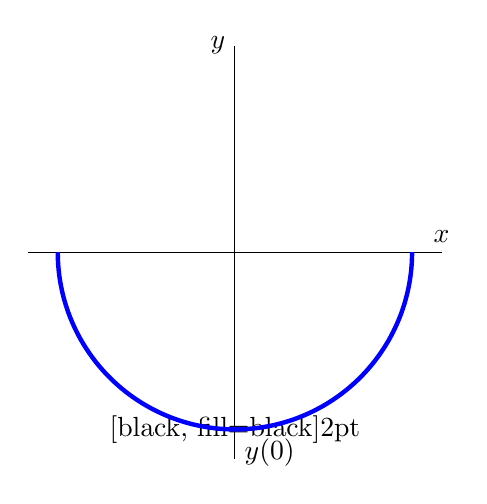
\begin{tikzpicture}[xscale=0.75,yscale=0.75]
	\draw[-{\seta}] (-3.5,0) -- (3.5,0) node[above] {$x$};
	\draw[-{\seta}] (0,-3.5) -- (0,3.5) node[left] {$y$};
	\draw[] (0,-3) node {\tikzcircle[black, fill=black]{2pt}};
	\draw[] (0,-3) node[below right] {$y(0)$};
  \draw[samples=100,ultra thick,domain=0:180,smooth,variable=\t,blue] plot ({3*cos(\t)},{-3*sin(\t)});
\end{tikzpicture}
	& 
	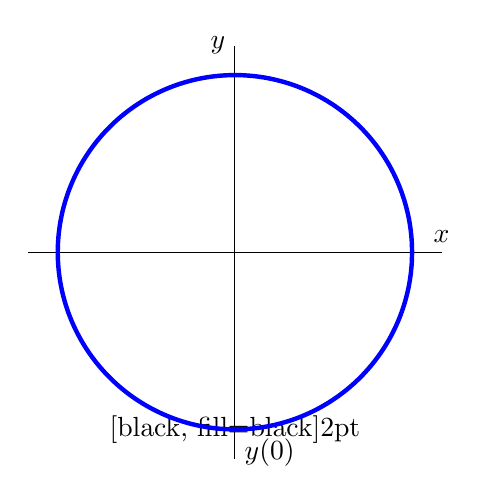
\begin{tikzpicture}[xscale=0.75,yscale=0.75]
		\draw[-{\seta}] (-3.5,0) -- (3.5,0) node[above] {$x$};
		\draw[-{\seta}] (0,-3.5) -- (0,3.5) node[left] {$y$};
		\draw[] (0,-3) node {\tikzcircle[black, fill=black]{2pt}};
		\draw[] (0,-3) node[below right] {$y(0)$};
	  \draw[samples=100,ultra thick,domain=0:360,smooth,variable=\t,blue] plot ({3*cos(\t)},{-3*sin(\t)});
	\end{tikzpicture}

	\\
Solution of the initial-value problem
	& Integral curve for the initial-value problem
\end{tabular}
\end{center}





\end{example}



	\begin{exercises}
		% Topics:
		% 
	\begin{problist}
	\prob Check that curves of the form $x^2 + y^2 = C$ satisfy the differential equation $\dfrac{dy}{dx} = -\dfrac{x}{y}$.
	
	
	\prob Is the piecewise-defined function
	$$
	y(x) = \begin{cases}
 		-x^2 & \text{ if } x< 0 \\
 		x^2 & \text{ if } x \geq 0		
	\end{cases}
	$$
	a solution of the differential equation $xy'-2y=0$ on $(-\infty,\infty)$?
	
	
	\prob Consider the differential equation
	$$ y^{(4)} - 8y^{3)} + 26 y'' - 40y'+25y=0.$$
	
	\begin{enumerate}
		\item Is $y=4 e^{2x}\sin(x)$ a solution?
		\item Is $y=-8 x e^{2x}\cos(x)$ a solution?
		\item For the two function above, if they are solutions, what are initial conditions of the form
			\begin{itemize}
				 \item[] $y(0) =$
				 \item[] $y'(0) =$
				 \item[] $y''(0) =$
				 \item[] $y'''(0) =$
			\end{itemize}
			that the solution satisfies?
	\end{enumerate}


	\prob Consider the functions
	\begin{align*}
		f(x) & = 3x + x^2 	& g(x) & = e^{-7x} \\
		h(x) & = \sin(x) 	& j(x) & = \sqrt{x} \\
		k(x) & = 8 e^{3x}	& \ell(x) & = -2 \cos(x)
	\end{align*}
	
	Match each differential to one or more functions which are solutions.
	
	\begin{enumerate}
		\item $y'=3y$
		\item $y''+9y'+14y=0$
		\item $y''+y=0$
		\item $2x^2y'' + 3xy'=y$
	\end{enumerate}
	
	
	
	\prob Consider the differential equation $u' = -2(u-10)$.
	
	\begin{enumerate}
		\item Check that the curves of the form $u = 10 + C e^{-2t}$ satisfy the differential equation.
		\item Sketch one solution of the differential equation.
		\item Sketch all the integral curves for the differential equation.
		\item What is the difference between a solution passing through the point $(1,20)$ and an integral curve passing through the same point?
	\end{enumerate}


	\prob Consider the differential equation $y'\big( 3y^2-1\big) = 1$.
	
	\begin{enumerate}
		\item Check that the curves of the form $y^3-y=x+C$ satisfy the differential equation.
		\item Sketch the solution of the differential equation that passes through $(1,1)$.
		\item Sketch the integral curve for the differential equation that passes through $(1,1)$.
		\item What is the difference between a solution passing through the point $(1,1)$ and an integral curve passing through the same point?
		\item Repeat (b)--(d) with the points $(1,0)$ and $(1,-1)$ instead of $(1,1)$.
	\end{enumerate}


	\prob Consider the ODE \quad $y'(t) = \big(y(t)\big)^2$ \quad .
	One of these two graphs {\bf cannot} describe the solution. 
	Which one? 
	
	
	\begin{center}
	\begin{tikzpicture}
		\draw[-{\seta}] (-1,0) -- (3,0) node[above] {$t$};
		\draw[-{\seta}] (0,-3) -- (0,1) node[left] {$y$};
		\draw[ultra thick,domain=0.5:2.5,smooth,variable=\x,blue] plot ({\x},{(\x*\x-5)/3-1});
	\end{tikzpicture}
	\hfil
	\begin{tikzpicture}
		\draw[-{\seta}] (-1,0) -- (3,0) node[above] {$t$};
		\draw[-{\seta}] (0,-3) -- (0,1) node[left] {$y$};
		\draw[ultra thick,domain=0.5:2.5,smooth,variable=\x,blue] plot ({\x},{-((\x-3.5)^2)/4-0.25});
	\end{tikzpicture}	
	\end{center}

	\prob We seek a first-order ordinary differential equation \quad $y' = f(\pmb{y})$ \quad whose solutions satisfy
	$$
	\begin{cases}
	y(x)  \mbox{ is concave up if } y < 1 \\
	y(x) \mbox{ is concave down if } y > 1
	\end{cases}
	$$
	%
	Write down or graph a function $f(y)$ that would produce such solutions.

	
	\end{problist}
\end{exercises}

\end{module}



\begin{lesson}
	\Title{Solutions of Differential Equations}

%	\Heading{Objectives}
%	\begin{itemize}
%		\item The second step in Mathematical modelling is to construct a representation of how the team will be attempting to solve the problem.
%		\item Create a mind map of the problem. This is a structured way to brainstorm possible solutions and their requirements.
%	\end{itemize}
%	
%	\Heading{Motivation} 
%
%\begin{annotation}
%	\begin{goals}
%	\Goal{Extra Reading}
%	Math Modelling: Getting started and getting solutions, Bliss-Fowler-Galluzzo
%	
%	\hfill \qrcode{https://m3challenge.siam.org/resources/modeling-handbook}	
%	\end{goals}
%\end{annotation}
%	\Heading{Extra Reading} \href{https://m3challenge.siam.org/resources/modeling-handbook}{Math Modelling: Getting started and getting solutions, Bliss-Fowler-Galluzzo}
%
\end{lesson}




\newpage

\question

Which of these shows solutions of $y' = (x-1)(x+1) = x^2 - 1$ ?

\newlength{\len}
%\setlength{\len}{120pt}
%\begin{tabular}{ccc}
%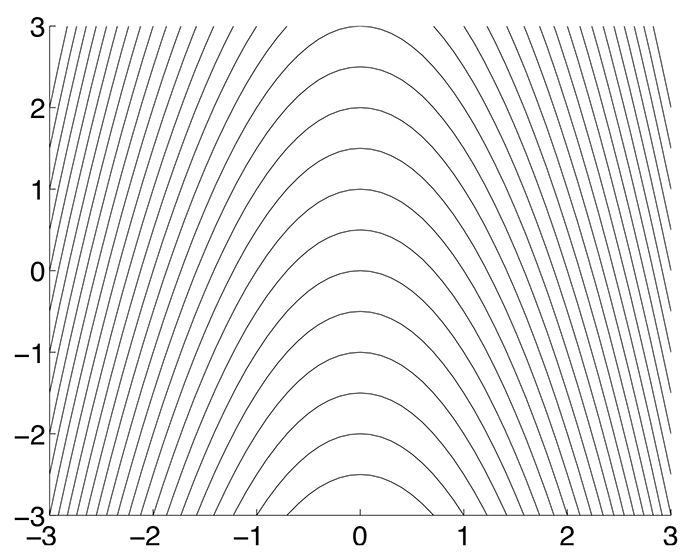
\includegraphics[width=\len]{images/module8-figs-6-small.png}
%	& 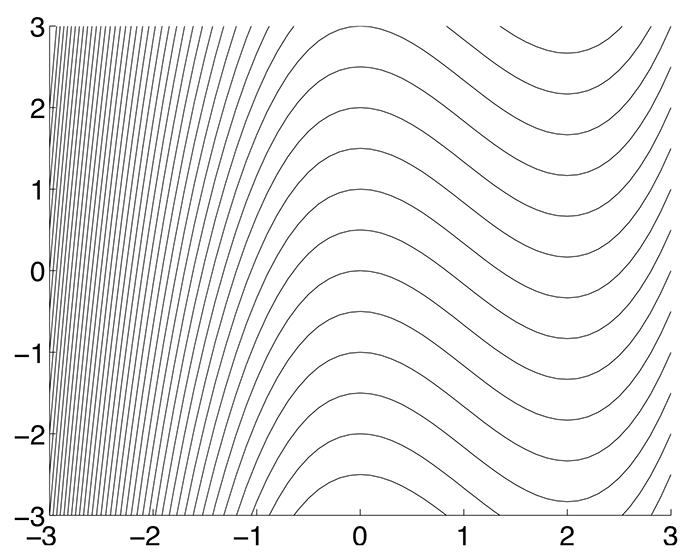
\includegraphics[width=\len]{images/module8-figs-3-small.png}
%	& \includegraphics[width=\len, page=2]{images/module8-figs-2-small.png} \\
%A & B & C \\[15pt]
%%
%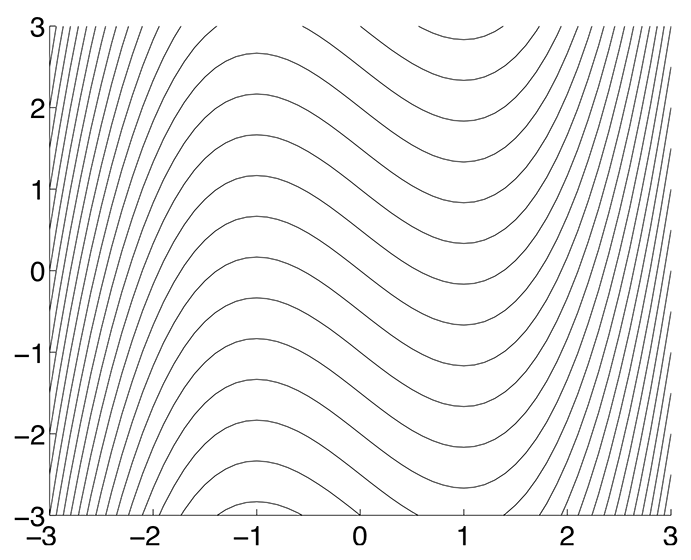
\includegraphics[width=\len]{images/module8-figs-1-small.png}
%	& 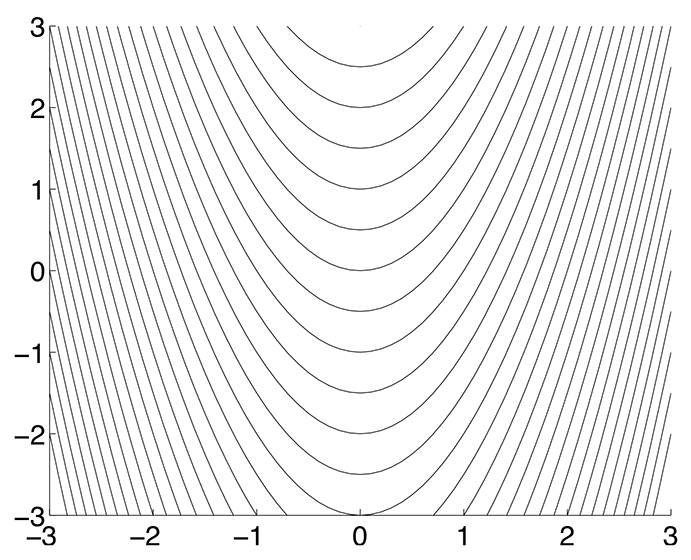
\includegraphics[width=\len]{images/module8-figs-5-small.png}
%	& 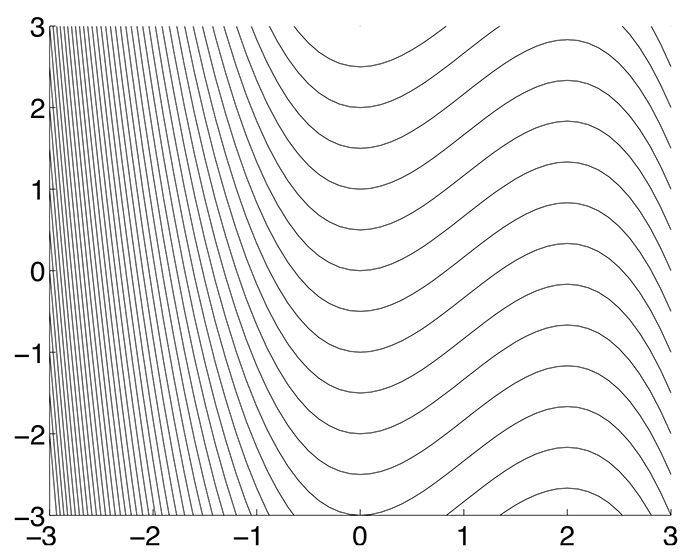
\includegraphics[width=\len]{images/module8-figs-4-small.png} \\
%D & E & F \\
%\end{tabular}


\def\modeightA{
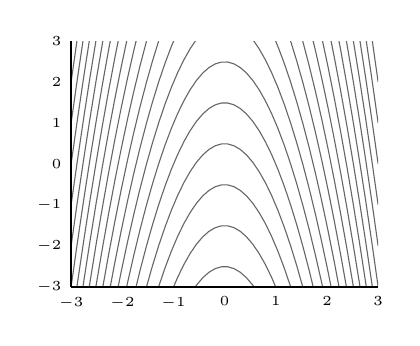
\begin{tikzpicture}[scale=0.65,yscale=0.8]
    \begin{scope}
	    \clip (-3,-3) rectangle (3,3);
		\foreach \k in {-9,-7, ..., 31} {
	      \draw[samples=50,domain=-3:3,variable=\x,color=gray!80!black] plot ({\x},{(\k-3*(\x*\x))/2});
	    }
    \end{scope}
    \draw[thick] (-3,-3) -- (-3,3);
    \draw[thick] (-3,-3) -- (3,-3);
    \foreach \k in {-3,-2, ..., 3} {
      \draw ({\k,-3}) node[below] {\tiny $\k$};
      \draw ({-3,\k}) node[left] {\tiny $\k$};
    }
\end{tikzpicture}
}

\def\modeightB{
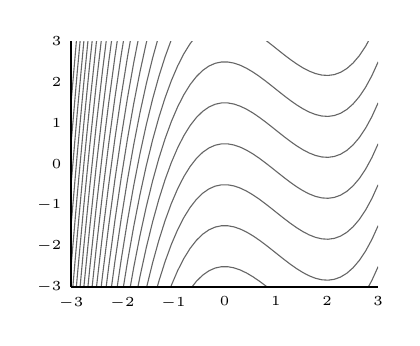
\begin{tikzpicture}[scale=0.65,yscale=0.8]
    \begin{scope}
	    \clip (-3,-3) rectangle (3,3);
		\foreach \k in {-9,-7, ..., 39} {
	      \draw[samples=50,domain=-3:3,variable=\x,color=gray!80!black] plot ({\x},{((\x*\x*\x)/3-(\x*\x)+\k/2)});
    	}
    \end{scope}
    \draw[thick] (-3,-3) -- (-3,3);
    \draw[thick] (-3,-3) -- (3,-3);
    \foreach \k in {-3,-2, ..., 3} {
      \draw ({\k,-3}) node[below] {\tiny $\k$};
      \draw ({-3,\k}) node[left] {\tiny $\k$};
    }
\end{tikzpicture}
}

\def\modeightC{
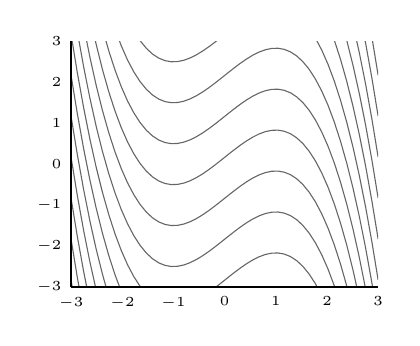
\begin{tikzpicture}[scale=0.65,yscale=0.8]
    \begin{scope}
	    \clip (-3,-3) rectangle (3,3);
		\foreach \k in {-15,-13, ..., 29} {
	      \draw[samples=50,domain=-3:3,variable=\x,color=gray!80!black] plot ({\x},{-(((\x+1)*(\x+1)*(\x+1))/3-((\x+1)*(\x+1))+\k/2)});
    	}
    \end{scope}
    \draw[thick] (-3,-3) -- (-3,3);
    \draw[thick] (-3,-3) -- (3,-3);
    \foreach \k in {-3,-2, ..., 3} {
      \draw ({\k,-3}) node[below] {\tiny $\k$};
      \draw ({-3,\k}) node[left] {\tiny $\k$};
    }
\end{tikzpicture}
}

\def\modeightD{
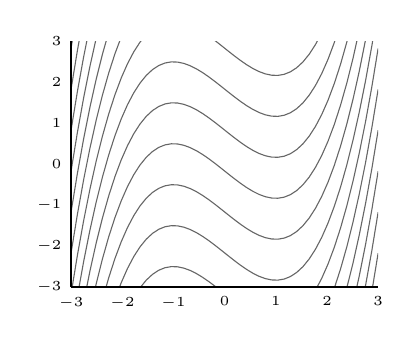
\begin{tikzpicture}[scale=0.65,yscale=0.8]
    \begin{scope}
	    \clip (-3,-3) rectangle (3,3);
		\foreach \k in {-15,-13, ..., 29} {
	      \draw[samples=50,domain=-3:3,variable=\x,color=gray!80!black] plot ({\x},{(((\x+1)*(\x+1)*(\x+1))/3-((\x+1)*(\x+1))+\k/2)});
    	}
    \end{scope}
    \draw[thick] (-3,-3) -- (-3,3);
    \draw[thick] (-3,-3) -- (3,-3);
    \foreach \k in {-3,-2, ..., 3} {
      \draw ({\k,-3}) node[below] {\tiny $\k$};
      \draw ({-3,\k}) node[left] {\tiny $\k$};
    }
\end{tikzpicture}
}

\def\modeightE{
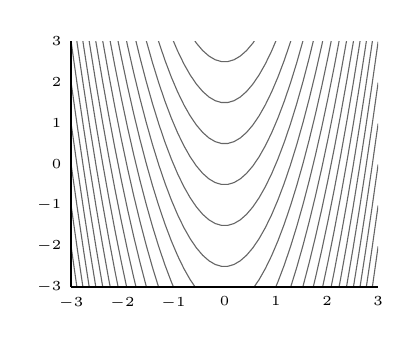
\begin{tikzpicture}[scale=0.65,yscale=0.8]
    \begin{scope}
	    \clip (-3,-3) rectangle (3,3);
		\foreach \k in {-9,-7, ..., 31} {
	      \draw[samples=50,domain=-3:3,variable=\x,color=gray!80!black] plot ({\x},{-(\k-3*(\x*\x))/2});
	    }
    \end{scope}
    \draw[thick] (-3,-3) -- (-3,3);
    \draw[thick] (-3,-3) -- (3,-3);
    \foreach \k in {-3,-2, ..., 3} {
      \draw ({\k,-3}) node[below] {\tiny $\k$};
      \draw ({-3,\k}) node[left] {\tiny $\k$};
    }
\end{tikzpicture}
}

\def\modeightF{
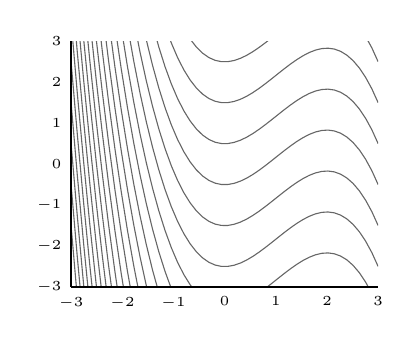
\begin{tikzpicture}[scale=0.65,yscale=0.8]
    \begin{scope}
	    \clip (-3,-3) rectangle (3,3);
		\foreach \k in {-9,-7, ..., 39} {
	      \draw[samples=50,domain=-3:3,variable=\x,color=gray!80!black] plot ({\x},{(-(\x*\x*\x)/3+(\x*\x)-\k/2)});
    	}
    \end{scope}
    \draw[thick] (-3,-3) -- (-3,3);
    \draw[thick] (-3,-3) -- (3,-3);
    \foreach \k in {-3,-2, ..., 3} {
      \draw ({\k,-3}) node[below] {\tiny $\k$};
      \draw ({-3,\k}) node[left] {\tiny $\k$};
    }
\end{tikzpicture}
}


\begin{tabular}{ccc}
\modeightA
	& \modeightB
	& \modeightC \\
A & B & C \\[15pt]
%
\modeightD
	& \modeightE
	& \modeightF \\
D & E & F \\
\end{tabular}



\bookonlynewpage


\question

We seek a first-order ordinary differential equation 
\quad $y' = f(x)$ \quad 
whose solutions satisfy
$$
\begin{cases}
y(x)  \mbox{ is increasing if } x<2 \\
y(x) \mbox{ is decreasing if } 2 < x < 4 \\
y(x) \mbox{ is increasing if } x > 4
\end{cases}
$$
%
Write down or graph an $\pmb{f(x)}$ that would produce such solutions.




\bookonlynewpage

\question

Consider the ODE \quad $y'(t) = \big(y(t)\big)^2$ \quad .
Which of the following is true?
	
\begin{parts}
	\item $y(t)$ must always be positive
	\item $y(t)$ must always be negative \\[5pt]

	\item $y(t)$ must always be decreasing
	\item $y(t)$ must always be increasing
\end{parts}




\bookonlynewpage

\question Consider the differential equation $2xy'=y$.
	
	\begin{parts}
		\item Check that the curves of the form $y^2 + C x = 0$ satisfy the differential equation.
		\item Sketch one solution of the differential equation.
		\item Sketch all the integral curves for the differential equation.
		\item What is the difference between a solution passing through the point $(1,-1)$ and an integral curve passing through the same point?
	\end{parts}








%%%%%%%%%%%%%%%%%%%%%%%%%%%%%%%%%%%%%%%%%%%%%%%%%%%%%%%%%%%%%%%%%%%%%%%%
%		Slope Fields



%%%%%%%%%%%%%%%%%%%%%%%%%%%%%%
%
%  MODULE - Slope Fields
%
%%%%%%%%%%%%%%%%%%%%%%%%%%%%%%



\begin{module}{Slope Fields}
	%\Title{Slope Fields}
	\label{intro-slopefields}

	In this module you will learn
\begin{itemize}
	\item what is a slope field
	\item how to sketch a slope field
	\item to interpret a slope field
\end{itemize}

\hfill \\

As we saw in the previous module, once we have found a differential equation that models a situation, we often want to figure out what happens to the solution.

In this module, we will focus on getting an idea of the solutions and integral curves using what is called a \textbf{slope field}.





\begin{definition}[Slope field] Consider the equation $y' = f(x,y)$.
If we evaluate $f(x,y)$ over a rectangular grid of points, and we draw an arrow at each point $(x,y)$ of the grid with slope $f(x,y)$, then the collection of all the arrows is called a \emph{slope field}.
\end{definition}

\begin{graybox}
	
We can sketch Slope Fields with Wolfram Alpha.

For a differential equation $\dfrac{dy}{dx} = f(x,y)$, we need to input
\begin{itemize}
	\item Vector Field: $(1, f(x,y))$.
\end{itemize}

\url{http://www.wolframalpha.com/input/?i=slope+field}
\hfill \qrcode{http://www.wolframalpha.com/input/?i=slope+field}	
\end{graybox}





\begin{example}
Let us take an \hyperlink{sols-ex}{example from the previous module}.

Consider the initial-value problem
$$
\begin{cases}
	\dfrac{dy}{dx}=-\dfrac{x}{y} \\
	y(0)=-3
\end{cases}
$$

We can use this definition to sketch the slope field for the differential equation $ \dfrac{dy}{dx} = -\dfrac{x}{y}$.

We now sketch this slope field with Desmos:

\url{https://www.desmos.com/calculator/scmz6ps0or} \hfill \qrcode{https://www.desmos.com/calculator/scmz6ps0or}

Now notice that the arrows have the slope of a solution. This means that solutions will be tangent to the arrows, so we can \emph{roughly} trace the solution by following the arrows.

Below, we did just that starting with the point $(0,-3)$.

\setlength{\len}{175pt}
\begin{center}
%\begin{figure}
%\includegraphics*[width=\len]{images/module9-slopefield-ex1.png}
%\hfil
\begin{tabular}{ccc}
\includegraphics*[width=\len]{images/module9-slopefield-ex1-sol.png}
 & & 
\includegraphics*[width=\len]{images/module9-slopefield-ex1-intcurve.png}\\
approximated solution & & approximated integral curve
\end{tabular}
%\caption{Slope Field for the differential equation $\frac{dy}{dx} = -\frac{x}{y}$.
%\label{mod9-slopefield1}
%\end{figure}
\end{center}

\textbf{\textcolor{orange}{Important. }} Remember that this gives us only an approximation of the solution and integral curve. From the approximation, we can tell that the solution seems circular, but we still need to show that it is so.

\end{example}



%\setlength{\len}{150pt}
%\hspace{-1.35cm}\begin{tabular}{ccc}
%\includegraphics*[width=\len]{figures/0101_dirfield_rocket.png}
%	& \includegraphics*[width=\len]{figures/0101_intcurves_rocket.png} 
%	& \includegraphics*[width=\len]{figures/0101_rocket_pos.png} \\
%Direction field for $u$
%	& Approximations of $u$
%	& Solution $u(t)$
%\end{tabular}


%
%This particular one is:
%\href{http://www.wolframalpha.com/input/?i=direction+field+calculator&f1=%7B1%2C-9.8*x-0.75*y%2B10%7D%2Fsqrt(1%2B(-9.8*x-0.75*y%2B10)%5E2)&f=VectorPlot.vectorfunction%5Cu005f%7B1%2C-9.8*x-0.75*y%2B10%7D%2Fsqrt(1%2B(-9.8*x-0.75*y%2B10)%5E2)&f2=x&f=VectorPlot.vectorplotvariable1%5Cu005fx&f3=0&f=VectorPlot.vectorplotlowerrange1%5Cu005f0&f4=2&f=VectorPlot.vectorplotupperrange1_2&f5=y&f=VectorPlot.vectorplotvariable2%5Cu005fy&f6=0&f=VectorPlot.vectorplotlowerrange2%5Cu005f0&f7=4&f=VectorPlot.vectorplotupperrange2%5Cu005f4}{\tt Click Here}
%\hfill \qrcode{http://www.wolframalpha.com/input/?i=direction+field+calculator&f1=%7B1%2C-9.8*x-0.75*y%2B10%7D%2Fsqrt(1%2B(-9.8*x-0.75*y%2B10)%5E2)&f=VectorPlot.vectorfunction%5Cu005f%7B1%2C-9.8*x-0.75*y%2B10%7D%2Fsqrt(1%2B(-9.8*x-0.75*y%2B10)%5E2)&f2=x&f=VectorPlot.vectorplotvariable1%5Cu005fx&f3=0&f=VectorPlot.vectorplotlowerrange1%5Cu005f0&f4=2&f=VectorPlot.vectorplotupperrange1_2&f5=y&f=VectorPlot.vectorplotvariable2%5Cu005fy&f6=0&f=VectorPlot.vectorplotlowerrange2%5Cu005f0&f7=4&f=VectorPlot.vectorplotupperrange2%5Cu005f4}



\begin{video}
\begin{itemize}
	\item \qrvideo{https://youtu.be/MI2xCwBekX4}
	\item \qrvideo{https://youtu.be/8Amgakx5aII}
\end{itemize}	
\end{video}



	\begin{exercises}
		% Topics:
		% 
	\begin{problist}
	\prob Use Wolfram Alpha, Desmos, or another software to sketch the slope field for the following differential equations. Then roughly trace different solutions.
	\begin{enumerate}
		\item $y'=2y-x$
		\item $y'=xy$
		\item $y'=\cos(y)$
		\item $y'=\frac12+\cos(y)$
		\item $y'=1+\cos(y)$
		\item $y'=2+\cos(y)$
		\item $y'=\sin(xy)$
		\item $y'=\tan(x+y)$
	\end{enumerate}
	
	\prob Sketch a slope field for the following differential equation
	$$ y'=f(x,y)$$
	where 
	$$
	f(x,y) = \begin{cases}
 		-x & \text{ if } x< 1 \\
 		y & \text{ if } x \geq 1		
	\end{cases}
	$$

	\prob Sketch a slope field for the following differential equation
	$$ y'=f(x,y)$$
	where the function $f(x,y)$ satisfies all of the following properties:
	\begin{enumerate}
		\item $f(x,y)$ is continuous
		\item $f(x,y) > 0$ when $x>1$ and $y>1$
		\item $f(x,y) < 0$ when $x<-1$ and $y<-1$
		\item $f(x,y)$ depends only on $x$ when $x<-1$ and $y>1$
		\item $f(x,y)$ depends only on $y$ when $x>1$ and $y<-1$
	\end{enumerate}
	
	
	\prob 
		\begin{enumerate}
			\item On the slope field from the previous problem, show that there must exist a smooth continuous curve with horizontal lines.

			\item Show that the curve divides the $(x,y)$ plane in two parts.

		\end{enumerate}
	
	


	\prob Consider a differential equation 
	$$ y'=f(x,y)$$
	where the solutions satisfy
	$$ \lim_{x\to \infty} y(x) = 1.$$

	\begin{enumerate}
		\item What property must the slope field satisfy?

		\item Sketch a possible slope field for this differential equation.
	\end{enumerate}
	
	\end{problist}
\end{exercises}

\end{module}



\begin{lesson}
	\Title{Slope Fields}

	\Heading{Objectives}
	\begin{itemize}
		\item The second step in Mathematical modelling is to construct a representation of how the team will be attempting to solve the problem.
		\item Create a mind map of the problem. This is a structured way to brainstorm possible solutions and their requirements.
	\end{itemize}
	
	\Heading{Motivation} 

\begin{annotation}
	\begin{goals}
	\Goal{Extra Reading}
	Math Modelling: Getting started and getting solutions, Bliss-Fowler-Galluzzo
	
	\hfill \qrcode{https://m3challenge.siam.org/resources/modeling-handbook}	
	\end{goals}
\end{annotation}
	\Heading{Extra Reading} \href{https://m3challenge.siam.org/resources/modeling-handbook}{Math Modelling: Getting started and getting solutions, Bliss-Fowler-Galluzzo}

\end{lesson}




\newpage

\question
\begin{minipage}{.7\textwidth}
	A catapult throws a projectile into the air and we track the height (in metres) of the projectile from the ground as a function $y(t)$, where $t$ is the time (in seconds) that elapsed since the object was launched from the catapult. \\

	Then, the slope fields for $y(t)$ and $y'(t)$ are shown below:
\end{minipage}\hfill
\begin{minipage}{100pt}
	\includegraphics*[width=100pt]{images/module9-catapult.pdf}	
\end{minipage}






\setlength{\len}{200pt}
\begin{tabular}{cc}
\includegraphics*[height=\len]{images/module9-y.png}
	& \includegraphics*[height=\len]{images/module9-yprime.png} \\
Slope field for $y(t)$
	& Slope field for $y'(t)$
\end{tabular}

\hfill {\footnotesize(These slope fields were created using WolframAlpha)} \\

\begin{parts}
	\item On the slope field, sketch a \emph{possible} solution.	
	\item Consider the graph of $y(t)$. Does it form a parabola? Justify your answer.
\end{parts}

\begin{annotation}
	\begin{Goals}
		Students should think about the initial conditions.
		What is a possible value for $y(0)$? What is a possible value for $y'(0)$?
		Then sketch a possible solution that starts at those values. \\
		
		The equilibrium in the slope field for $y'(t)$ is called \emph{terminal velocity}. Some students might be able to identify it.
	\end{Goals}
\end{annotation}





\bookonlynewpage



\question Sketch the slope field for the following differential equations. 

\begin{parts}
	\item $y'=x$

\begin{annotation}
	\begin{Goals}
		The goal is not to be very accurate, but to capture the symmetry of each of these slope fields.
	\end{Goals}
	
\end{annotation}

	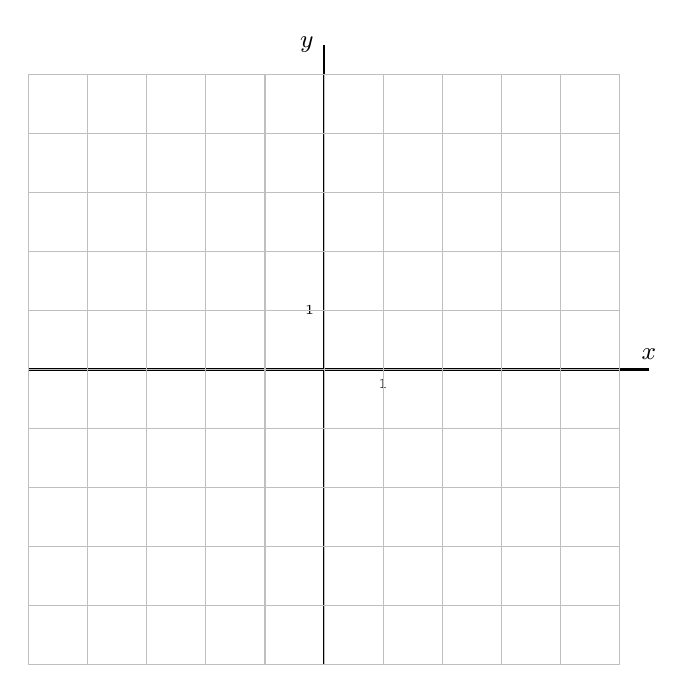
\begin{tikzpicture}[xscale=0.75,yscale=0.75]
		\draw[thick,-{\seta}] (-5,0) -- (5.5,0) node[above] {\small $x$};
		\draw[thick,-{\seta}] (0,-5) -- (0,5.5) node[left] {\small $y$};
		\draw[] (1,0) node[below] {\tiny 1};
		\draw[] (0,1) node[left] {\tiny 1};
		\draw[step=1,lightgray,thin] (-5,-5) grid (5,5);
	\end{tikzpicture}
	
	
\vfil	
	
	\item $y'=y^2$	

	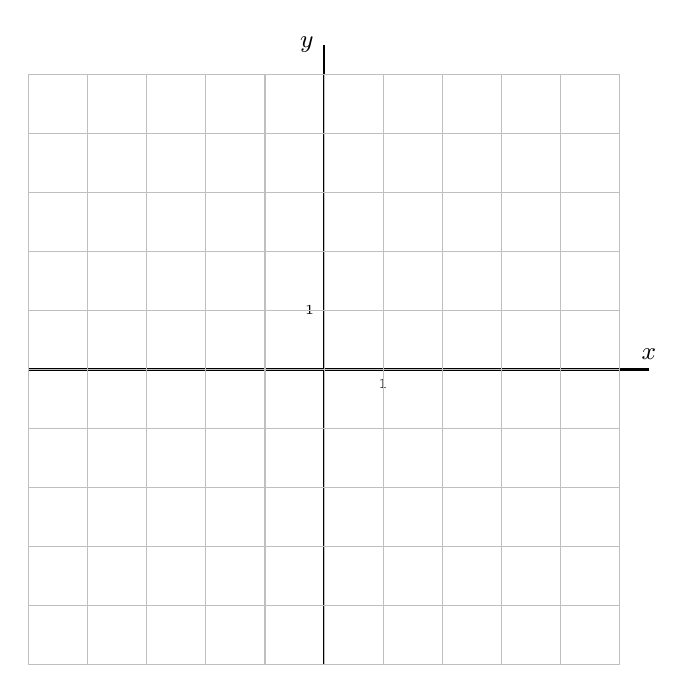
\begin{tikzpicture}[xscale=0.75,yscale=0.75]
		\draw[thick,-{\seta}] (-5,0) -- (5.5,0) node[above] {\small $x$};
		\draw[thick,-{\seta}] (0,-5) -- (0,5.5) node[left] {\small $y$};
		\draw[] (1,0) node[below] {\tiny 1};
		\draw[] (0,1) node[left] {\tiny 1};
		\draw[step=1,lightgray,thin] (-5,-5) grid (5,5);
	\end{tikzpicture}

\end{parts}



\bookonlynewpage

\question Consider the following slope fields:


\setlength{\len}{150pt}
\begin{tabular}{ccc}
	\includegraphics*[height=\len]{images/module9-graph1}
		& \includegraphics*[height=\len]{images/module9-graph2}
		& \includegraphics*[height=\len]{images/module9-graph3} \\
		(A) & (B) & (C) \\[10pt]
	\includegraphics*[height=\len]{images/module9-graph4}
		& \includegraphics*[height=\len]{images/module9-graph5}
		& \includegraphics*[height=\len]{images/module9-graph6} \\
		(D) & (E) & (F)
\end{tabular}

\hfill {\footnotesize(These slope fields were created using WolframAlpha)} \\


\begin{parts}
	\item Which slope field(s) corresponds to a differential equation of the form
		\qquad $y'=f(x)$ \qquad ?	

	\item Which slope field(s) corresponds to a differential equation of the form
		\qquad $y'=g(y)$ \qquad ?	

	\item Which slope field(s) corresponds to a differential equation of the form
		\qquad $y'=h(x+y)$ \qquad ?	

	\item Which slope field(s) corresponds to a differential equation of the form
		\qquad $y'=\kappa(x-y)$ \qquad ?	

	\item Which slope field(s) corresponds to a differential equation of the form
		\qquad $y'=1+\big( \ell(x,y) \big)^2$ \qquad ?	

	\item Which slope field(s) corresponds to a differential equation of the form
		\qquad $y'=1-\big( m(x,y) \big)^2$ \qquad ?	

\end{parts}

\begin{annotation}
	\begin{Goals}
		Students should be able to justify their choices	.
	\end{Goals}
	
\end{annotation}






\newpage



%%%%%%%%%%%%%%%%%%%%%%%%%%%%%%%%%%%%%%%%%%%%%%%%%%%%%%%%%%%%%%%%%%%%%%%%
%		Numerical Methods



%%%%%%%%%%%%%%%%%%%%%%%%%%%%%%
%
%  MODULE - Numerical Methods
%
%%%%%%%%%%%%%%%%%%%%%%%%%%%%%%



\begin{module}{Approximating Solutions}
	%\Title{Slope Fields}
	\label{Approximation}

	In this module you will learn
\begin{itemize}
	\item to approximate the solutions of differential equations
\end{itemize}

\hfill \\

We just learned to sketch a slope field and how to use it to sketch a rough approximation of a solution of a differential equation.

The method of ``following the arrows'' of a slope field, when formalized mathematically is called \textbf{\color{cyan}Euler's Method}. 

So let us start with an initial-value problem
$$
\begin{cases}
	y'(t) = f\big(t,y(t) \big) \\
	y(0) = y_0
\end{cases}
$$

The idea is to follow the directions given by the differential equation, so we know that
\begin{itemize}
	\item $y(0)=y_0$
	\item $y'(0) = f(0,y_0)$
\end{itemize}

This means that we have a starting point \quad {\color{cyan}$(0,y_0)$}.
We still need to decide the distance that we want to follow the arrow:
\begin{itemize}
	\item smaller distance: more accurate approximation, but will take more calculations
	\item longer distance: less accurate approximation, but will take fewer calculations
\end{itemize}

The typical way to decide is to set a parameter {\color{cyan}$\Delta t$}, that measures the distance we will travel in the $t$-axis.

\begin{center}
	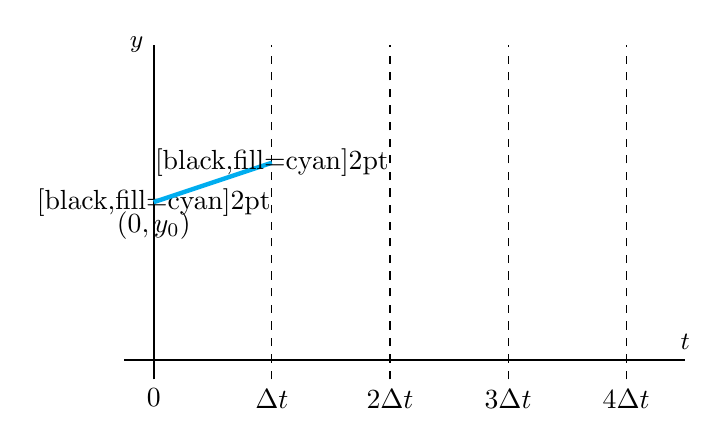
\begin{tikzpicture}[xscale=1.5]%,yscale=0.35]
		\draw[thick,-{\seta}] (-0.25,0) -- (4.5,0) node[above] {\small $t$};
		\draw[thick,-{\seta}] (0,-0.25) -- (0,4) node[left] {\small $y$};
		\foreach \t in {2,...,4} {
			\draw[dashed] (\t,-0.25) -- (\t,4);
			\draw[] (\t,-0.25) node[below] {$\t \Delta t$};
		}
		\draw[] (0,-0.25) node[below] {$0$};	
		\draw[dashed] (1,-0.25) -- (1,4);
		\draw[] (1,-0.25) node[below] {$\Delta t$};	
		\draw[] (0,2) node{\tikzcircle[black,fill=cyan]{2pt}};
		\draw[] (0,2) node[below] {$(0,y_0)$};
	%	\draw[ultra thick, lightblue] (5,2) node {\tikzcircle[black,fill=magenta]{2pt}}-- (3,6) node {\tikzcircle[black,fill=navy]{2pt}};
		\draw[ultra thick, cyan,-{\setam}] (0,2) -- (1,2.5);
		\draw[] (1,2.5) node{\tikzcircle[black,fill=cyan]{2pt}};
	\end{tikzpicture}
\end{center}

This way we find our second point \quad {\color{cyan} $(\Delta t,y_1)$} \quad where:
$$
\frac{y_1 - y_0}{\Delta t} = \text{ slope of the arrow }= f(0,y_0)
\quad \Rightarrow \quad
	y_1 = y_0 + f(0,y_0) \Delta t $$

We continue in this way to find more points \quad {\color{cyan} $(t_i, y_i)$}:
\begin{center}
	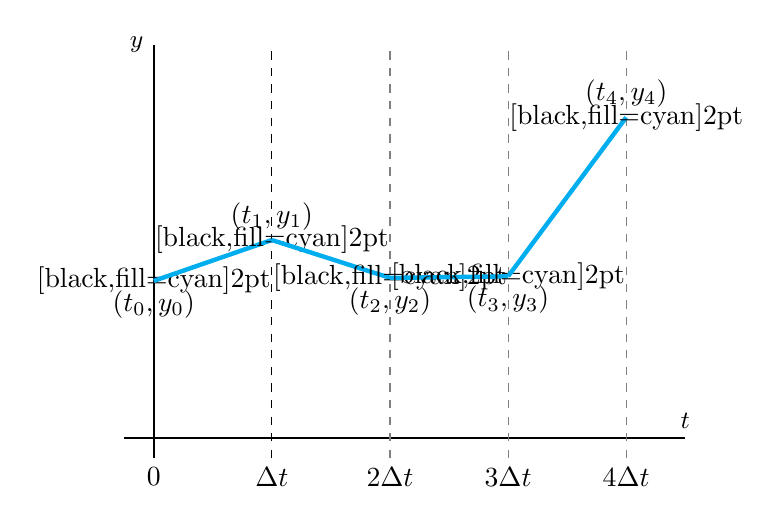
\begin{tikzpicture}[xscale=1.5]%,yscale=0.35]
		\draw[thick,-{\seta}] (-0.25,0) -- (4.5,0) node[above] {\small $t$};
		\draw[thick,-{\seta}] (0,-0.25) -- (0,5) node[left] {\small $y$};
		\foreach \t in {2,...,4} {
			\draw[dashed, gray] (\t,-0.25) -- (\t,5);
			\draw[] (\t,-0.25) node[below] {$\t \Delta t$};
		}
		\draw[] (0,-0.25) node[below] {$0$};	
		\draw[dashed] (1,-0.25) -- (1,5);
		\draw[] (1,-0.25) node[below] {$ \Delta t$};	
		\draw[] (0,2) node{\tikzcircle[black,fill=cyan]{2pt}};
		\draw[] (0,2) node[below] {$(t_0,y_0)$};
		\foreach \t in {1,...,4} {
			\draw[ultra thick, cyan,-{\setam}] ({\t-1},{2.25+(\t-2)^3/4-(\t-1)^2/2+(\t-1)/1.3}) -- ({\t},{2.25+(\t-1)^3/4-\t^2/2+\t/1.3});
			\draw[] (\t,{2.25+(\t-1)^3/4-\t^2/2+\t/1.3}) node{\tikzcircle[black,fill=cyan]{2pt}};
		}
		\foreach \t in {1,4} {
			\draw[] (\t,{2.25+(\t-1)^3/4-\t^2/2+\t/1.3}) node[above] {$(t_{\t},y_{\t})$};	
		}
		\foreach \t in {2,3} {
			\draw[] (\t,{2.25+(\t-1)^3/4-\t^2/2+\t/1.3}) node[below] {$(t_{\t},y_{\t})$};	
		}

	\end{tikzpicture}
\end{center}


\begin{definition}[Euler's Method]
	Let $y'(t) = f(t,y)$ be a first-order differential equation. 
	The \emph{Euler approximation} to the initial value problem $y'(t)=(f(t,y)$ and $y(t_0)=y_0$ with step size $\Delta t$ is the sequence of points $(t_i,y_i)$ given by $(t_0,y_0)$ if $i=0$ and 
	\begin{itemize}
		\item $t_i = t_{i-1}+\Delta t$
		\item $y_i = y_{i-1} +  f\big(t_{i-1},y_{i-1}\big) \Delta t$.
	\end{itemize}
	
	The method used to generate $(t_i,y_i)$ is called \emph{Euler's Method}.
\end{definition}


\begin{example}
Consider the initial-value problem
$$
\begin{cases}
y'(t) = \sin(y)+t \\
y(-3)=2
\end{cases}
$$

\begin{minipage}{.65\textwidth}
Then, we can follow Euler's Method with $h=0.5$ to obtain:
\begin{itemize}
	\item $y_0=2$
	\item $y_1 = 2 + \frac12 \big(\sin(2) -3\big) \approx 0.95$
	\item $y_2 = 0.95 + \frac12 \big(\sin(0.95) -2.5\big) \approx 0.1$
	\item $y_3 = 0.1 + \frac12 \big(\sin(0.1) -2\big) \approx -0.85$
\end{itemize}

%\begin{center}
%%	\begin{figure}[hbtp]
%	\includegraphics*[width=200pt]{images/module10-Euler.pdf}
%%	\caption{Graph of the Euler approximation and the slope field for the differential equation using desmos.}
%%	\end{figure}
%\end{center}
	
\begin{minipage}{220pt}
Here is the link to the desmos graph: 
\begin{itemize}
	\item \href{https://www.desmos.com/calculator/kkgj5jhggd}{https://www.desmos.com/calculator/kkgj5jhggd} %\hfill \qrcode{https://www.desmos.com/calculator/kkgj5jhggd}
\end{itemize}
\end{minipage}
\hfill
\begin{minipage}{55pt}
	\qrcode{https://www.desmos.com/calculator/kkgj5jhggd}
\end{minipage}
\end{minipage}
\hfill
\begin{minipage}{150pt}
	\includegraphics*[width=150pt]{images/module10-Euler-small.pdf}
\end{minipage}	

\end{example}


\begin{video}
\begin{itemize}
	\item \qrvideo{https://youtu.be/q87L9R9v274}
	\item \qrvideo{https://youtu.be/g3Xw1r7QGOE}
	\item Euler's Method helping to take a person to the Moon \hfill \qrcode{https://youtu.be/v-pbGAts_Fg}
\end{itemize}	
\end{video}






	\begin{exercises}
	
	\begin{problist}
	
	\prob \label{approx:comp}For the following initial-value problems, approximate their solution with different values of $\Delta t$ and compare with their exact solutions. 
	\begin{enumerate}
		\item $y'=-y+5+t$, $y(0) = 4,5,6$
		\item $y'=y+5-t$, $y(0) = -4$
		\item $y'=(t-y)\sin(y)$, $y(0)=-1$
		\item $\displaystyle y'=\frac{y+3t}{1+t^2}$, $y(0)=-1,1$
	\end{enumerate}
	
	\textbf{Hint. } Write a computer program that does the approximation for you.
	
	
	\prob Consider the differential equation
	$$ y'=-\frac{x}{y}.$$
	\begin{enumerate}
		\item Sketch a slope field for this differential equation.
		\item Use Euler's Method to approximate the solution for some values of $\Delta x$ and for some initial conditions.
		\item Does Euler Method do a good job approximating the solution?
	\end{enumerate}
	
	\begin{annotation}
	\begin{Goals}
		There is a singularity at $y=0$, so the method will behave erratically when it goes across that line.
			\href{https://www.desmos.com/calculator/5swjyrxvtr}{https://www.desmos.com/calculator/5swjyrxvtr} \hfill \qrcode{https://www.desmos.com/calculator/5swjyrxvtr}
	\end{Goals}
	\end{annotation}
	
	
	
	
	\prob In this module, we derived Euler's Method. One of the main steps was obtaining the equation
	$$\frac{y_1-y_0}{\Delta t} = \text{slope of the arrow}.$$
	
	In Euler's Method, we used the slope at the beginning of the arrow. We can derive a new Method where we use the slope at the end of the arrow. 
	
	\begin{enumerate}
		\item Find a formula and the algorithm for this new method.
		\item Use this method with to approximate the solution of $y'=-y+5+t$, $y(0) = 4,5,6$ and compare the results with your results from question \ref{approx:comp}.
		\item Which of these two methods gives a better approximation?
		\item In your opinion, which of these two methods is better? Why?
	\end{enumerate}
	
	
	
	
	
	
	
	
	
	
	
	\prob Consider an initial-value problem with solution $y(t)$. If we want to find an approximation for $t \in [0,T]$, we define the error of the approximation $\{y^{\Delta t}_i\}$ by
	\begin{equation}\tag{E}\label{error} 
		E(\Delta t) = \big| y(T) - y^{\Delta t}_N \big|,
	\end{equation}
	where $T = N \Delta t$.
	
	\begin{enumerate}
		\item For the initial-value problems from the previous question, study what happens when the value of $\Delta t$ decreases.
		\item What do you expect to happen as $\Delta t$ converges to $0$?
		\item Estimate how fast Euler's method converges. Find a value of $p$ such that
			$$ E(\Delta t) \leq C (\Delta t)^p,$$
		where the constant $C$ changes for each ODE, but doesn't change if you keep the same ODE but change only the value of $\Delta t$.
%		\item In fact, when using Euler's method on a computer, there are more approximations that are subtler. For example, the computer approximates every number that you write and it also approximates every operation that the method needs. This means that the real error of the approximation 
	\end{enumerate}
	

	\prob Using Euler's Method with a step size of $\Delta t = 0.05$, and keeping only three digits throughout your computations, determine the approximations at $T=0.2, 0.3, 0.4$ for each of the following initial-value problems.
	\begin{enumerate}
		\item $y'=-y+5+t$, $y(0) = 4$
		\item $y'=y+5-t$, $y(0) = -4$
	\end{enumerate}
	Compare the results with what you obtained for problem \ref{approx:comp}. Where do the differences come from?
	
	\prob Round-off errors become important when the value of $N$ is very large, which happens if we want a very accurate approximation. This means that the actual error \eqref{error} of the approximation has two components:
	$$ E(\Delta t) = f(\Delta t) + g(\Delta t), $$
	where
	\begin{itemize}
		\item $\displaystyle \lim_{\Delta t \to 0^+} f(\Delta t) = 0$ \hfill (approximation error)
		\item $\displaystyle \lim_{\Delta t \to \infty} f(\Delta t) = \infty$ \hfill (approximation error)
		\item $\displaystyle \lim_{\Delta t \to 0^+} g(\Delta t) = \infty$ \hfill (round-off error)
		\item $\displaystyle \lim_{\Delta t \to \infty} f(\Delta t) = 0$ \hfill (round-off error)
	\end{itemize}
	
	Answer the following questions and justify your answers based on these ideas.
	\begin{enumerate}
		\item Justify why the four limits above make sense.
		\item Does the approximation converge to the solution as $\Delta t \to 0$?
		\item Is there an optimal $\Delta t$ that gives the best possible approximation?
	\end{enumerate}
	
	

	
	
	\end{problist}
\end{exercises}
\end{module}



\begin{lesson}
	\Title{Approximating Solutions}

%	\Heading{Objectives}
%%	\begin{itemize}
%%		\item The second step in Mathematical modelling is to construct a representation of how the team will be attempting to solve the problem.
%%		\item Create a mind map of the problem. This is a structured way to brainstorm possible solutions and their requirements.
%%	\end{itemize}
%	
%	\Heading{Motivation} 
%
%\begin{annotation}
%	\begin{goals}
%	\Goal{Extra Reading}
%	Math Modelling: Getting started and getting solutions, Bliss-Fowler-Galluzzo
%	
%	\hfill \qrcode{https://m3challenge.siam.org/resources/modeling-handbook}	
%	\end{goals}
%\end{annotation}
%	\Heading{Extra Reading} \href{https://m3challenge.siam.org/resources/modeling-handbook}{Math Modelling: Getting started and getting solutions, Bliss-Fowler-Galluzzo}
%
\end{lesson}




\newpage

\question
	Consider the differential equation
	$$ y' = y - 2 .$$
	
\begin{parts}
	\item Use Euler's Method to find an approximation of the solution of this differential equation that passes through the point $(0,3)$.
	\item Find the solution of the differential equation with the same initial condition.

	\item Use Euler's Method to find an approximation of the solution of this differential equation that passes through the point $(0,1)$.
	\item Find the solution of the differential equation with the same initial condition.

	\item Compare the approximations with the actual solutions. Is there a property of the Euler's Method that you can infer?
	\item Explain in words why the Method satisfies that property.
	

\end{parts}

\begin{annotation}
	\begin{Goals}
		The goal is to have student's recognize that the Euler approximation ``curves slower'' than the actual solution.
		
		Students can explain in words why that is the case using the way the approximations are generated.
	\end{Goals}
\end{annotation}


\bookonlynewpage



\question
	Which differential equations will be approximated perfectly using Euler's Method?

\begin{annotation}
	\begin{Goals}
		The question is purposefully ambiguous.
		What do we mean by approximated perfectly?
		
		Ex: The IVP $y'=$ sign$(t)$ (assuming sign$(0)=1$) with $y(-5)=5$ has solution $y = |t|$ and it is captured with Euler's method if $\Delta t=\frac5k$ for any $k\in\mathbb{N}$. \\
		
		Once students discuss, they'll find ODE's of the form $y'= c$ for any constant. 
		
		Prompt them to find other types. Show them the example above only after they tried for a bit. 
		Then, let them revise their Conjecture.  \\
		
		Ex 2: $y'=f(y+t)$ with $y(0)=0$ and $f(z) = \lfloor z \rfloor$ is approximated perfectly if $\Delta t = 1$, but not if $\Delta t$ takes any other value.
		
	\end{Goals}
\end{annotation}








%\bookonlynewpage







%%%%%%%%%%%%%%%%%%%%%%%%%%%%%%%%%%%%%%%%%%%%%%%%%%%%%%%%%%%%%%%%%%%%%%%%
%
%		Chapter 3 -
%
%%%%%%%%%%%%%%%%%%%%%%%%%%%%%%%%%%%%%%%%%%%%%%%%%%%%%%%%%%%%%%%%%%%%%%%%
%
%
%\begin{topic}[First-Order Models]
%
%\end{topic}
%
%

%%%%%%%%%%%%%%%%%%%%%%%%%%%%%%%%%%%%%%%%%%%%%%%%%%%%%%%%%%%%%%%%%%%%%%%%
%		Modelling with ODEs


\begin{module}{Modelling with Differential Equations}
	%\Title{Slope Fields}
	\label{model-odes}

	In this module you will learn
\begin{itemize}
	\item how to start modelling a physical phenomenon into a differential equation
\end{itemize}

\hfill \\


We started by studying some mathematical modelling in chapter 1. Then, we just used mathematical tools that we learned before. 

We now want to focus on mathematical models that arise from physical applications. These will often take the form of one or more differential equations.

The modelling of the situation will develop in a similar way.


\paragraph{\emph{Step 1.}} Defining the problem \\

As before, we should start by thinking about what our ultimate goal is. 
Once we settle on a goal, we define it as the function we want to study.

\begin{example}

\begin{minipage}{.7\textwidth}
In this module, we are going to think about the catapult problem from Module 9 - Slope Fields. \\

A catapult throws a projectile into the air.

Our goal is to track the height (in metres) of the projectile from the ground.

This means that we have a goal: to find the height of the projectile at every moment in time after it is launched.
\end{minipage}\hfill
\begin{minipage}{100pt}
	\includegraphics*[width=100pt]{images/module9-catapult.pdf}	
\end{minipage}
\hfill \\[10pt]

This means that we define
\begin{itemize}
	\item $y(t) = $ height of the projectile, in metres, $t$ seconds after it was launched from the catapult.
\end{itemize}

\end{example}

\hfill \\

\paragraph{\emph{Step 2.}} Building a mind map \\

A mind map will help us identify the notions that we want to include in our model.


\begin{example}

In the catapult example, since we decided to study the projectile's height, we need to find everything that affects its height.

\begin{center}
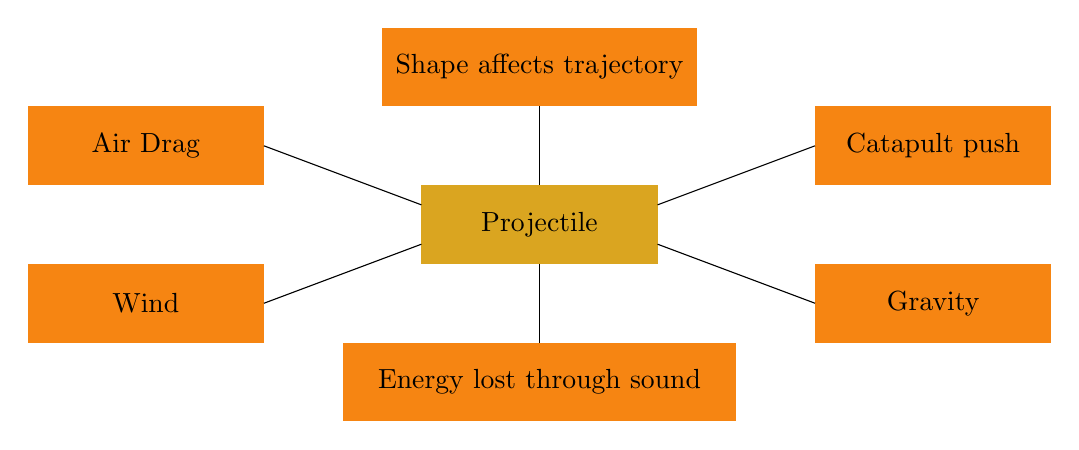
\begin{tikzpicture}
	\fill[color=Goldenrod] (0,0) rectangle (3,1) node[pos=.5] {\color{black}Projectile};
	\fill[color=BurntOrange] (5,1) rectangle (8,2) node[pos=.5] {\color{black}Catapult push};
	\fill[color=BurntOrange] (5,-1) rectangle (8,0) node[pos=.5] {\color{black}Gravity};
	\fill[color=BurntOrange] (-5,1) rectangle (-2,2) node[pos=.5] {\color{black}Air Drag};
	\fill[color=BurntOrange] (-5,-1) rectangle (-2,0) node[pos=.5] {\color{black}Wind};
	\fill[color=BurntOrange] (-1,-2) rectangle (4,-1) node[pos=.5] {\color{black}Energy lost through sound};
	\fill[color=BurntOrange] (-0.5,2) rectangle (3.5,3) node[pos=.5] {\color{black}Shape affects trajectory};
	\draw (3,0.75) -- (5,1.5);
	\draw (3,0.25) -- (5,-0.5);
	\draw (0,0.75) -- (-2,1.5);
	\draw (0,0.25) -- (-2,-0.5);
	\draw (1.5,0) -- (1.5,-1);
	\draw (1.5,1) -- (1.5,2);
\end{tikzpicture}
\end{center}

We can include more layers to these topics if we want.

\end{example}


\hfill \\

\paragraph{\emph{Step 3.}} Make assumptions \\

This is a fundamental step in any modelling endeavour. The real world is too complicated, so we make assumptions that simplify our model.

This has two main consequences:
\begin{enumerate}
	\item It makes our model simpler and easier to study;
	\item It creates constraints on our model: it is only valid under certain conditions.
\end{enumerate}

\begin{example}

Let us discuss the topics included in the mind map above:
\begin{itemize}
	\item Catapult Push -- the catapult pushes on the projectile for a small period of time when $t<0$. If we are considering only $t\geq 0$, then this will likely provide us with some starting conditions for the projectile
	\item Gravity -- The height of the projectile is affected by gravity. We have a choice to make:
	\begin{itemize}
		\item assume that the Earth is flat and gravity is constantly accelerating the projectile downwards;
		\item assume that the Earth is spherical and gravity is constantly accelerating the projectile towards the centre of the Earth;
		\item assume that the Earth is spherical and gravity is a force accelerating the projectile towards the centre of the Earth with a magnitude that decreases with the square of the distance to the centre of the Earth
		\item or other more complicated and more accurate models.
	\end{itemize}
	
	\item Air Drag -- air is making it hard for the projectile to move forward. We have another choice to make:
	\begin{itemize}
		\item assume that the air drag is a force that accelerates the projectile in the direction opposite to its movement and with magnitude proportional to its speed;
		\item assume that the air drag is a force that accelerates the projectile in the direction opposite to its movement and with magnitude proportional to the square of its speed;
		\item or other more complicated and more accurate models.
	\end{itemize}
\end{itemize}
	
I will leave it to you to think about the remaining three topics in the mind map. \\


We now need to make a decision about what to assume. \\

To keep this model simple, let us assume the following:
\begin{enumerate}
	\item The projectile's height will stay within a small range: $y(t) \in [0,100]$. Is this reasonable for a catapult?

		This means that we can consider the first of the gravitational models above: define gravitational acceleration as a constant $-g$.
		
	\item The projectile will not move very fast, so we can approximate the air drag to be directly proportional to the speed: define air drag acceleration as $\pm \gamma v$, where $\gamma>0$ is a constant that depends on the projectile and $v$ is the velocity of the projectile. Which sign should we have?

	\item Again, the projectile will not move very fast, so we can approximate the air drag to use only the vertical speed of the projectile: define air drag acceleration as $\pm \gamma v_y$, where $\gamma>0$ is a constant that depends on the projectile and $v_y$ is the vertical velocity of the projectile. Which sign should we have?

	\item The shape of the projectile will affect air drag in the form of the constant $\gamma>0$.

	\item Assume that for a medieval catapult (as in the drawing above), the other components are negligible.

\end{enumerate}

We come out of this step with some conditions for the validity of our model and some new constants and terms to use in our model.

\end{example}

\hfill \\

\paragraph{\emph{Step 4.}} Construct a model \\

This is the part where we put together the last three steps into one (or a system of) differential equations.

This should not be a difficult part if the last three steps were completed carefully.

\begin{example}

Summary of Steps 1--3:
\begin{itemize}
	\item \textbf{Goal:} study $y(t) = $ height of a projectile in metres, $t$ seconds after being released from a catapult
	\item \textbf{Forces:}
	\begin{itemize}
		\item Gravity: constant acceleration $-g$
		\item Air Drag: acceleration $\pm \gamma y'(t)$
	\end{itemize}
	\item \textbf{Conditions:}
	\begin{itemize}
		\item $y(t) \in [0,100]$
		\item Air drag should really by quadratic, but in this example we will consider this as an academic case.
	\end{itemize}
\end{itemize}

So the model we end up is:
$$
F_y = \substack{\text{vertical component}\\\text{of force}} = -g \pm \gamma y'.
$$

Now we bring a little bit of a Physics class into here: Newton's 2$^{\rm nd}$ Law states that \quad $F = m a$ \quad, so we obtain the model
$$m y''(t) =  -g \pm \gamma y'(t).$$
\end{example}



\paragraph{\emph{Step 5.}} Model Assessment

We just found a differential equation (model) for our situation. It is now time to test it to make sure that it behaves correctly.

For this step, we need to obtain a solution of the differential equation, either by solving it mathematically and finding a formula for the solution, or by approximating the solution numerically (see Module \ref{NumericalMethods}).

Then we need to check if the differential in one of several ways:
\begin{itemize}
	\item We can test it empirically: make an experiment and compare the results of the experiment with the results of the model
	\item We can test it mathematically: change the parameters and the initial conditions to make sure that we know how the model should behave and test some qualitative aspects of the model
\end{itemize}

\begin{important}
Even if the model passes all the tests, it might still not be correct.

Also, if it fails one test, it might mean that the model is incorrect, or that it has some limitations that are more subtle and we hadn't thought about them.	
\end{important}

\begin{example}
We have found the following model:
\begin{itemize}
	\item $y(t) = $ height of a projectile in metres, $t$ seconds after being released from a catapult
	\item It satisfies:
		$$m y''(t) =  -g + \gamma y'(t).$$
	(note that I chose the $+$ sign for the air drag component)

	\item Constraints:
	\begin{itemize}
		\item $y(t) \in [0,100]$;
		\item $\gamma >0$ is the drag constant: more air drag for larger values of $\gamma$;
	\end{itemize}
\end{itemize}	

This differential equation tells us what the second derivative, $y''(t)$, of $y(t)$ is given the first derivative $y'(t)$.
This means that to start solving the problem, we need to know what the initial values for $y'(t)$ and $y(t)$ are.

Need to know the starting conditions:
\begin{itemize}
	\item $y(t_0) = y_0$;
	\item $y'(t_0) = v_0$.
\end{itemize}

For this example, consider a situation where:
\begin{itemize}
	\item $g, \gamma >0$ can take any value.
	\item $y(0) = 0$;
	\item $y'(0) = g/\gamma > 0$;
\end{itemize}

The projectile is being catapulted from the ground with a positive velocity, so we expect it to go up for a while and then come back down to the ground.

What happens is 
$$
y''(0) = -g + \gamma y'(0) = 0,
$$
so the initial acceleration is 0, which means that the velocity is not changing.

The result is a function with constant velocity equal to its initial velocity:
\begin{itemize}
	\item $y(t) = \frac{g}{\gamma}t.$
\end{itemize}

This means that the height of the projectile keeps increasing, so the \emph{projectile never falls back to the ground}! \\

This means that there is a problem with our differential equation:
\begin{itemize}
	\item Is the model incorrect? 
	\item Is there a limitation on the initial velocity that we were not aware of?
\end{itemize}
\hfil

We must check our process again and correct it.
\end{example}




\paragraph{\emph{Step 6.}} Putting it all together in a report

We're not going to elaborate much on this step. For more on the subject, please check Module \ref{report}.





\begin{video}
\begin{itemize}
	\item \href{https://youtu.be/njg8xwMviGQ}{https://youtu.be/njg8xwMviGQ} \hfill \qrcode{https://youtu.be/njg8xwMviGQ}
	\item \href{https://youtu.be/nKDsJB8iwb0}{https://youtu.be/nKDsJB8iwb0} \hfill \qrcode{https://youtu.be/nKDsJB8iwb0}
\end{itemize}	
\end{video}


	\begin{exercises}
		% Topics:
		% 
	\begin{center}
		\includegraphics*[width=175pt]{images/module11-lake.pdf}
	\end{center}
	\begin{problist}
	\prob Model the pollution in a lake where water flows in and out at the same rate and incoming water is polluted with $2+\sin(2t)$ kg/L of pollutant, where $t$ is measured in years.
	
		
	\prob Construct a model for a population with a rate of growth proportional to its current size.
	
	\prob Find a model for a population that grows proportionally to its current size but with a variable proportion constant. This variable proportion constant should guarantee the following properties for the population:
	\begin{itemize}
		\item If the population is too large, then it should decrease;
		\item If the population is small, then it should increase.
	\end{itemize}
		
	
	\prob Improve the previous model by considering also a \emph{survivability threshold}: if the population is below this value, it should decrease and eventually become extinct.
		
	
	\prob Consider two competing populations, like cheetahs ($c(t)$) and lions ($\ell(t)$): two populations that do not hunt each other, but compete for the same food (prey). Create a model for these two populations that captures how the competition for food affects them.
	
	{\bf Hint. } It might be helpful to think about how one population would grow in the absence of the other; and how one population is affected by the competition of the other.

	\begin{center}
			\includegraphics*[width=150pt]{images/module11-stadium.pdf}
	\end{center}
		
	\prob People are in a stadium watching cricket match. When the match is over, people leave the stadium. 
	
	\begin{enumerate}
	\item Model the way people leave the stadium.
	
	To help you with this task, use the fact that in this situation, people behave like a fluid according to Torricelli's Law:
	
		\begin{center}
		\framebox{
		\begin{minipage}{6cm}
		\begin{center}
		The area of the region occupied by the fans decreases proportionally to the square root of the radius and also proportionally to the size of the exit.
		\end{center}
		\end{minipage}}
		\end{center}

	\item How do the parameters $\theta$ and $\alpha$ affect the total time it will take for the stadium to empty?
	\end{enumerate}
	
	\begin{center}
		\includegraphics*[width=150pt]{images/module11-pool.pdf}
	\end{center}
	
	
	\prob Consider the pool in the figure. The goal is to track the amount of chlorine in the water for one Summer month. At the beginning of the month, the pool is full and contains 150g of chlorine uniformly mixed in the water. Consider evaporation and rain. To make the model simpler, assume that water evaporates with the chlorine.
	
	
	
	\prob After solving the core exercise \ref{pendulum} below, we find a property of this model. 
	\begin{enumerate}
		\item The constants $g$ and $L$ (length of the string) appear only has $\frac{g}{L}$. What does this imply?
		\item We are sending a mission to the Moon and we need to know how a 1m long pendulum behaves on the Moon. To test it, we need to build on Earth a pendulum that behaves in the same way. How long should the length of the string be on Earth?
	\end{enumerate}
	

	\prob After solving the core exercise \ref{pendulum} below, construct a model for the same problem considering string tension.
	\begin{enumerate}
		\item Show that you obtain the same model that you get while disregarding tension.
		\item Explain why this makes sense.
	\end{enumerate}
	
	\begin{center}
		\includegraphics*[width=150pt]{images/module11-ant_tunnel.pdf}
	\end{center}
	
	\prob 	An ant queen, known affectionately as Aunty Ant, is commissioning a construction assessment
	for a new tunnel.  Aunty Ant's worker ants only know one way to construct a tunnel: they grab some dirt in their pincers,
	walk the dirt out of the tunnel, deposit it, and then return to grab more dirt.
	
	Prepare a report which uses differential equations to address the following construction scenarios.  Include a
	description of how you modelled the scenario and a graph of tunnel-length vs.~worktime.
	Also make sure to define any variables and constants you are using.

	\begin{enumerate}
		\item One tireless worker is assigned dig the tunnel.  The worker walks the same speed
			whether she is carrying dirt or not.
		\item One tireless worker is assigned to dig the tunnel, but she can walk twice as fast
			when she is not carrying dirt as when she is carrying dirt.
		\item Aunty Ant really wants the tunnel to progress linearly after the first
			day of construction (that is, the graph of tunnel-depth vs.~time after
			the first day should be a straight line).  She will give you full control over
			how many workers are devoted to the tunnel at any given time.
		\item (Optional) A single ant is assigned to dig the tunnel, but she gets fatigued
			the farther she walks.  Her speed after walking a total distance of $k$ units is $1/k$.

	\end{enumerate}


	\prob 	The alien world of Robotron is inhabited by billions of tiny nanobots.  These nanobots
	all share a common source of power, and their speed is directly proportional to the
	total amount of energy shared among all the nanobots. 

	One day the nanobots decide to beam their energy into space.  They all form lines,
	march to the edge of their colony, and send a tiny portion of their shared energy into
	space.  Since the nanobots are very polite, after an individual nanobot has sent its energy
	into space, it moves aside and lets the next nanobot take a turn.

	\begin{enumerate}
		\item Suppose the nanobots live in a tube with an opening at only one end.  Come
			up with a differential equation to model the amount of energy left in the nanobot
			colony over time.
		\item How does your model change if the nanobots live in a disk where energy can be launched
			from anywhere on the perimeter?  What about a sphere?
		\item Newton's law of cooling states that the rate of change of temperature of an object is
			proportional to the difference between the object's temperature and the ambient (outside)
			temperature.  Does this law relate to your model for the nanobots?  If so, how?
	\end{enumerate}

	
	\end{problist}
\end{exercises}

\end{module}



\begin{lesson}
	\Title{Modelling with Differential Equations}

%	\Heading{Objectives}
%	\begin{itemize}
%		\item The second step in Mathematical modelling is to construct a representation of how the team will be attempting to solve the problem.
%		\item Create a mind map of the problem. This is a structured way to brainstorm possible solutions and their requirements.
%	\end{itemize}
%	
%	\Heading{Motivation} 
%
%\begin{annotation}
%	\begin{goals}
%	\Goal{Extra Reading}
%	Math Modelling: Getting started and getting solutions, Bliss-Fowler-Galluzzo
%	
%	\hfill \qrcode{https://m3challenge.siam.org/resources/modeling-handbook}	
%	\end{goals}
%\end{annotation}
%	\Heading{Extra Reading} \href{https://m3challenge.siam.org/resources/modeling-handbook}{Math Modelling: Getting started and getting solutions, Bliss-Fowler-Galluzzo}

\end{lesson}




\newpage


\begin{annotation}
	\begin{goals}
	\Goal{Pendulum and Rumours}
		This should take 2 lectures.
		
		Lecture 1. Focus on Pendulum problem. Students should finish it at home.
		
		
		Lecture 2. Rumour problem is more open-ended. 
		
		Students should follow the structure from chapter 1 to think about this problem.
	\end{goals}
\end{annotation}
		
		
		
\question \label{pendulum}
	A pendulum is swinging side to side. We want to model its movement.

\begin{minipage}{.7\textwidth}
\begin{parts}
	\item Define the problem. Which function(s) do we want to find in the end?
	\item Build a mind map.
	\item Make assumptions. Remember to use your mind map to help structure the problem.
	\item Construct a model. You should end up with one (or more) differential equations. 
	
	Remember that there are some Physics principles that can help you (e.g. Newton's 2$^{\rm nd}$ Law, Conservation of Energy, Linear Momentum, and Angular Momentum, Rate of Change is Rate in $-$ Rate out).
	\item Assess your model:
	\begin{enumerate}
		\item Find one test that your model passes.
		\item Find one test that your model fails.
	\end{enumerate}
	
\end{parts}
\end{minipage}\hfill
\begin{minipage}{100pt}
	\includegraphics*[width=100pt]{images/module11-pendulum.pdf}	
\end{minipage}







\begin{annotation}
	\begin{goals}
		Students will mostly likely identify the goal as finding the position of the ball $\vec{r}(t) = \big( x(t) , y(t) \big)$. That's fine!
		
		Later, in Step 3, try to guide the students to recognize the following:
		\begin{itemize}
			\item Rope is massless (negligible)
			\item Rope doesn't bend (negligible)
			\item So can assume that the rope is rigid. How does that affect the position of the ball?
			\item No friction (negligible)
			\item \textbf{Important:} Students always focus on string tension. One can consider it, but it all cancels out. It's one of the exercises of the module (above). For the lecture, don't consider tension.
		\end{itemize}
		
		Then on Step 4, guide students to recognize that they actually only need to find a model for the angle, because the position of the ball really only depends on the angle $\theta(t): \vec{r}\big(\theta(t)\big)$
				
	\end{goals}
\end{annotation}







\bookonlynewpage

\hfill



\bookonlynewpage

\question \label{rumour} Model the spreading of a rumour through the students of a school.






%%%%%%%%%%%%%%%%%%%%%%%%%%%%%%%%%%%%%%%%%%%%%%%%%%%%%%%%%%%%%%%%%%%%%%%%
%		Solvable Types of ODEs: Separable, First-Order Linear, Exact (?)


\begin{module}{Solvable Types of ODEs}
	%\Title{Separable ODEs}

	\label{model-odes}

	In this module you will learn
\begin{itemize}
	\item to identify specific types of differential equations that can be solved rigorously
	\item how to solve these types of differential equations
\end{itemize}

\hfill \\

We just learned how to model a situation and end up with a differential equation.
We will now focus on solving differential equations. 

There are a few different techniques that depend on the differential equation. 

\hfill

\begin{submodule}{Separable Differential Equations}

\begin{definition}[Separable ODE]
A differential equation is called \emph{separable} if it has the form
$$
g(y) y'(t) = h(t),
$$
that is if we can separate all the $y$'s into the left-hand side and the all the $t$'s into the right-hand side of the equation. Observe that the $y$'s on the left hand side must all be multiplied by $y'(t)$. 
\end{definition}


\subparagraph{\textcolor{cyan}{Method of solution. }} The idea to solve this type of DEs is simple:
\begin{enumerate}[label={\bf \arabic*. } ]
\item Integrate both sides with respect to $t$:
$$
\int g(y) y'(t) \, dt = \int h(t) \, dt
$$

\item Change variables on the left-hand side to $u = y(t)$, so $du = y'(t) dt$ and we get
$$
\int g(u) \, du = \int h(t) \, dt.
$$

\item Solve both integrals and we obtain a solution, usually in implicit form:
$$
G(u) = H(t) + C.
$$

\item To finish, recall that $u=y(t)$, so we obtain
$$
G\big(y(t)\big) = H(t) + C.
$$
\end{enumerate}

\begin{important}
	Observe that the solution is given in implicit form. In general, when using this technique, the solution $y(t)$ will be given in implicit form, so there is still some work ahead to find an explicit formula for $y(t)$.	
\end{important}



\def\arcsinh{\rm arcsinh\ }
\begin{example}
The shape $y(x)$ of a free falling chain under its own weight, called a catenary, satisfies the differential equation:
$$
y''(x) = \frac1a \sqrt{1+\big(y'(x)\big)^2}.
$$

It doesn't seem to be a \textbf{\color{Red!70!black}separable equation}, but if we can define $z(x) = y'(x)$, which satisfies
$$
z'(x) = \frac1a \sqrt{1+\big(z(x)\big)^2}
\qquad \Leftrightarrow \qquad \frac{1}{\sqrt{1+\big(z(x)\big)^2}} z'(x) = \frac1a.
$$

This is now clearly in the form of a \emph{\color{Red!70!black}separable ODE}. \\

We can solve it using the method described above: we need to solve
$$
\int \frac{1}{\sqrt{1+z^2}}\,dz \quad = \quad \int \frac1a \,dx \quad = \quad \frac{x}{a} + C_1
$$
The integral on the left can be solved using a hyperbolic substitution $z = \sinh u$:
$$
\int \frac{1}{\sqrt{1+z^2}}\,dz = \int 1 \, du = u = \arcsinh z.
$$
This means that the solution satisfies
$$
\arcsinh z = \frac{x}{a} + C_1 
\qquad \Leftrightarrow \qquad z = \sinh \left(\frac{x}{a} + C_1 \right).
$$

Now recall that $z(x) = y'(x)$, so we need to integrate $z(x)$ to obtain the catenary curve $y(x)$:
$$
y(x) = \int z(x) \, dx = a \cosh \left(\frac{x}{a} + C_1\right) + C_2.
$$

To find $C_1$ and $C_2$, we use the fact that $y'(0)=0$:
$$
y(x) = a \cosh \frac{x}{a}  + C_2.
$$
(the constant $C_2$ moves the curve up or down, so it doesn't change the shape).
\end{example}


\begin{video}
\begin{itemize}
	\item \href{https://youtu.be/txtFH89HwOA}{https://youtu.be/txtFH89HwOA} \hfill \qrcode{https://youtu.be/txtFH89HwOA}
	\item \href{https://youtu.be/8xG_Xg6X2MQ}{https://youtu.be/8xG\_Xg6X2MQ} \hfill \qrcode{https://youtu.be/8xG_Xg6X2MQ}
	\item \href{https://youtu.be/ZE1Agfkhr28}{https://youtu.be/ZE1Agfkhr28} \hfill \qrcode{https://youtu.be/ZE1Agfkhr28}
\end{itemize}	
\end{video}

\end{submodule}

\hfill \\

\begin{submodule}{First-Order Linear Differential Equations}

\begin{definition}[First-Order Linear ODE]
A differential equation is called \emph{first-order linear} if it has the form
$$
y'(t) + p(t) y(t) = f(t),
$$
that is if we can separate all the $y$'s into the left-hand side and the all the $t$'s into the right-hand side of the equation. Observe that the $y$'s on the left hand side must all be multiplied by $y'(t)$. 
\end{definition}


The idea to solve this type of DEs is to transform it into the result of a product rule. \\


\begin{example}
Consider the following \textbf{\color{Red!70!black}first-order linear ODE}
$$
t^2 \frac{dy}{dt} + 2t y = \sin t.
$$

Observe that the left-hand side of the DE is the result of the product rule:
$$
\frac{d}{dt} \bigg[ t^2 y \bigg] = \sin t.
$$
So  we can integrate both sides with respect to $t$ to obtain
$$
t^2 y = - \cos t + C 
\quad \Leftrightarrow \quad y = -\frac{\cos t}{t^2} + \frac{C}{t^2}.
$$
\end{example}


Now let us look at another example, where the left-hand side of the ODE is not in the form of the result of a product rule, but can be transformed into one.


\begin{example}
Consider the \textbf{\color{Red!70!black}first-order linear ODE}
\begin{equation}\tag{$\star$}\label{eq:intfact_1}
\frac{dy}{dt} + \frac12 y = \frac13 e^{\frac t3}.
\end{equation}
%which passes through the point $(0,1)$.


Again, the ``trick'' is to look at this equation and realize that the left-hand side can look like the result of the product rule.
It's not obvious that this can be done (yet!), but if we multiply the whole ODE by the function
$$
e^{\frac{t}{2}},
$$
then we obtain
$$
e^{\frac t2} \frac{dy}{dt} + \frac12e^{\frac t2} y = \frac13 e^{\frac t2} e^{\frac t3}
$$
and now the left-hand side is the result of a product rule
$$
\frac{d}{dt}\left[e^{\frac t2} y \right] = \frac13e^{\frac 56 t}.
$$

We integrate both sides to obtain
$$
e^{\frac t2} y = \frac13 \frac65 e^{\frac56 t} + c
$$
thus
$$
y %= \frac25 e^{\frac56 t-\frac12t} + c e^{-\frac t2} 
	= \frac25 e^{\frac t3} + c e^{-\frac t2}.
$$

\end{example}


This last example required us to come up with a function to multiply the ODE so that it becomes of the right form: with a left-hand side that is the result of the product rule.

This function is called the \textbf{\color{cyan}integrating factor}.

Let us now see how we can find this function in more detail.


\begin{example}
Consider the same ODE \eqref{eq:intfact_1}:
\begin{equation}\tag{$\star$}
\frac{dy}{dt} + \frac12 y = \frac13 e^{\frac t3}.
\end{equation}

So we multiply both sides of the equation with an unknown function $\mu(t)$, called the \textbf{\color{cyan}integrating factor}:
\begin{equation}\tag{\#}\label{eq:intfactor2}
\mu(t) \frac{dy}{dt} + \frac12 \mu(t) y = \frac13 \mu(t) e^{\frac t3}.
\end{equation}

And we find which $\mu(t)$ makes the left-hand side equal to the product rule:
$$
\frac{d}{dt} \big[ \mu(t) y \big] 
	= \mu(t) \frac{dy}{dt} + \frac{d \mu(t)}{dt} y,
$$
and this needs to equal the left-hand side:
$$
\mu(t) \frac{dy}{dt} + \frac{d \mu(t)}{dt} y = \mu(t) \frac{dy}{dt} + \frac12 \mu(t) y
\qquad \Leftrightarrow \qquad
	\mu'(t) = \frac12 \mu(t).
$$

We now need to solve this equation for $\mu(t)$. Fortunately, this is a \textbf{\color{cyan}separable ODE}:
\begin{align*}
\mu'(t) = \frac12 \mu(t) \quad
	& \Leftrightarrow \quad \frac{\mu'(t)}{\mu(t)} = \frac12 \\
	& \Leftrightarrow \quad \ln |\mu(t)| = \frac t2  + A\\
	& \Leftrightarrow \quad \mu(t) = a e^{\frac t2},
\end{align*}
where $a = e^A$.

We say that the function $\mu(t) = e^{\frac t2}$ is an \textbf{\color{cyan}integrating factor} for the equation \eqref{eq:intfact_1}.
Observe that we chose $a=1$ ($A=0$), because we only need one function $\mu(t)$ that satisfies our condition $\mu' = \frac12 \mu$, we don't need to find all possible solutions. \\


After finding the integrating factor $\mu(t)$, the rest of the solution is the same as in the previous example.
%
%The equation \eqref{eq:intfactor2} then becomes
%$$
%e^{\frac t2} \frac{dy}{dt} + \frac12e^{\frac t2} y = \frac13 e^{\frac t2} e^{\frac t3}
%$$
%or equivalently
%$$
%\frac{d}{dt}\left[e^{\frac t2} y \right] = \frac13e^{\frac 56 t}.
%$$
%
%We integrate both sides to obtain
%$$
%e^{\frac t2} y = \frac13 \frac65 e^{\frac56 t} + c
%$$
%thus
%$$
%y %= \frac25 e^{\frac56 t-\frac12t} + c e^{-\frac t2} 
%	= \frac25 e^{\frac t3} + c e^{-\frac t2}.
%$$
\end{example}


Now that we have a good idea of the method needed to solve these ODEs, let us tackle the general equation.


\subparagraph{\color{cyan}Method of solution. } This method is also known as the \textbf{\color{cyan}Method of the Integrating Factor}. 
\begin{enumerate}[label={\bf \arabic*. } ]
\item Multiply both sides by $\mu(t)$, the integrating factor:
$$
\mu(t) \frac{dy}{dt} + p(t)\mu(t) y = \mu(t) g(t).
$$

Note that we don't know what this function is yet. So it is just a placeholder for a function we will find next.

\item Find function $\mu(t)$ which satisfies
$$
\mu'(t) = p(t) \mu(t).
$$

This is a \textbf{\color{cyan}separable ODE}, so we can solve it:
$$
\mu(t) = A e^{\int p(t) \, dt}.
$$

We only need one function $\mu(t)$, not the general one, so we take $A=1$ to get
$$
\mu(t) = e^{\int p(t) \, dt}.
$$

\item Observe that $\mu(t)$ satisfies
$$
\mu(t) p(t) = \mu'(t),
$$
so we use this in the equation:
$$
\frac{d}{dt} \big[ \mu(t) y \big] = \mu(t) g(t).
$$

\item Integrate the equation:
$$
\mu(t) y = \int \mu(t) g(t) \, dt + c,
$$
which means that the solution is
$$
y = \frac{1}{\mu(t)} \left[ \int \mu(t) g(t) \, dt + c \right],
$$
where 
$$
\mu(t) = e^{\int p(t) \, dt}.
$$

\end{enumerate}

\begin{important}
	Observe that the solution is given in explicit form. This is always the case with this type of ODEs.
	
	Also, be careful to add the integration constant as soon as you integrate, so that in the end you will have a term $\frac{c}{\mu(t)}$.
\end{important}


\begin{video}
\begin{itemize}
	\item \href{https://youtu.be/ezhi3E_bdvk}{https://youtu.be/ezhi3E\_bdvk} \hfill \qrcode{https://youtu.be/ezhi3E_bdvk}
	\item \href{https://youtu.be/VdD26Iy4Bkk}{https://youtu.be/VdD26Iy4Bkk} \hfill \qrcode{https://youtu.be/VdD26Iy4Bkk}
	\item \href{https://youtu.be/GIpOcHNK7eQ}{https://youtu.be/GIpOcHNK7eQ} \hfill \qrcode{https://youtu.be/GIpOcHNK7eQ}
\end{itemize}	
\end{video}

\end{submodule}

%\hfill \\


	\begin{exercises}

	\begin{problist}
	\prob Solve the differential equation $\displaystyle \ln(t) y' + \frac{1}{t}y = 3$.
	
	\prob Decide whether the following differential equations are separable, first-order linear, both, or neither. If they are of one type, solve it.
	\begin{enumerate}
		\item $\displaystyle (t^2+4) y'(t) = \frac{2t}{y^2}$
		\item $\displaystyle \frac{1}{t^2} y'(t) = 2$
		\item $\displaystyle \frac{dy}{dx} = \sqrt{y} (x+1)^2$
		\item $\displaystyle y'(t) = t + y$
		\item $\displaystyle y'(t) = t + y^2$
		\item $\displaystyle y'(t) = \frac{t}{y}$
		\item $\displaystyle y'(t) = -\frac{1}{t} y$
		\item $\displaystyle y'(t) = 1 - 4t - \frac5t y$
		\item $\displaystyle y'(t) = 5t - 2t y$
		\item $\displaystyle y'(t) = 2 + \cos^2(y)$
		\item $\displaystyle e^{-t} y'(t) - e^{-t} y = 3e^{2t}$
	\end{enumerate}
	
	\prob Decide whether the following statements are true or false. Give an explanation or a counterexample.
	
	\begin{enumerate}
		\item There are differential equations that are both separable and first-order linear.
		\item There are differential equations that are separable, but are not first-order linear.
		\item There are differential equations that are first-order linear, but not separable.
		\item There are first-order differential equations that are neither separable nor linear.
		\item All first-order linear differential equations have solutions defined in the whole real line.
	\end{enumerate}
	
	
	\prob Consider the differential equation
	$$ y' - \frac{y}{2(x+4)} = \frac{1}{2(x+4)} $$
	\begin{enumerate}
		\item Find the general solution.
		\item Find the solution with initial condition $y(0)=-5$.
		\item What is the domain of the previous solution?
		\item Find the solution with initial condition $y(-5)=-5$.
	\end{enumerate}


	\prob Even though the following differential equation is not linear, find its general solution:
		$$ 2 \ln(x) e^{2y} y'(x) + \frac{e^{2y}}{x} = 4x^3.$$

	
	\end{problist}
\end{exercises}


%	\Heading{Textbook}	
%	\Heading{Objectives}
%	\begin{itemize}
%		\item Bla bla bla	
%	\end{itemize}
%	
%	\Heading{Motivation} 


\end{module}


\begin{lesson}
	\Title{Solvable Types of Differential Equations}

%	\Heading{Objectives}
%	\begin{itemize}
%		\item The second step in Mathematical modelling is to construct a representation of how the team will be attempting to solve the problem.
%		\item Create a mind map of the problem. This is a structured way to brainstorm possible solutions and their requirements.
%	\end{itemize}
%	
%	\Heading{Motivation} 
%
%\begin{annotation}
%	\begin{goals}
%	\Goal{Extra Reading}
%	Math Modelling: Getting started and getting solutions, Bliss-Fowler-Galluzzo
%	
%	\hfill \qrcode{https://m3challenge.siam.org/resources/modeling-handbook}	
%	\end{goals}
%\end{annotation}
%	\Heading{Extra Reading} \href{https://m3challenge.siam.org/resources/modeling-handbook}{Math Modelling: Getting started and getting solutions, Bliss-Fowler-Galluzzo}

\end{lesson}




\newpage

\question 
	Decide whether the following differential equations are separable, first-order linear, both, or neither. If they are of one of the solvable types, solve it.

\begin{parts}
	\item $\displaystyle\theta''(t) = \frac{g}{L} \sin\big(\theta(t)\big)$
	\item $\displaystyle P'(t) = r P(t) \left( 1 - \frac{P(t)}{K} \right)$
	\item $\displaystyle v'(t) = -g - \frac{\gamma}{m} v(t)$
	\item $\displaystyle y'(t) = -gt - \frac{g}{m} y(t) + 10$
\end{parts}











\bookonlynewpage


\question Consider a differential equation $y' = f(t,y)$ with the following slope field.

\begin{center}
	\includegraphics*[width=200pt]{images/module12-dirfield.pdf}
\end{center}

\begin{parts}
	\item What are the equilibrium solutions of the ODE?


\item Directly on the direction field above, sketch the solution of the problem
$$
\begin{cases}
y'=f(t,y) \\
y(0) = \dfrac14
\end{cases}
$$

\item From the direction field above, what is the type(s) of this ODE? Justify your answer.

\begin{enumerate}[label={\bf (\alph*)}]
\hfil 
\begin{minipage}{.3\textwidth}
\item separable. \\[-10pt]
\item of first-order and linear.
\end{minipage}
\hfil
\begin{minipage}{.4\textwidth}
\item autonomous. \\[-10pt]
\item none of the other options.
\end{minipage}
\end{enumerate}

\item Assume that $y=g(t)$ and $y=h(t)$ are two solutions of the differential equation with $g(0)<h(0)$, then

\hfill (select all the possible options)\\[-10pt]

\begin{enumerate}[label={\bf (\alph*)}]
\hfil 
\begin{minipage}{.2\textwidth}
\item $g(3) < h(3)$
\end{minipage}
\hfil
\begin{minipage}{.2\textwidth}
\item $g(3) = h(3)$
\end{minipage}
\hfil
\begin{minipage}{.2\textwidth}
\item $g(3) > h(3)$
\end{minipage}
\end{enumerate}

\end{parts}




\bookonlynewpage



\question
\begin{parts}
	\item Calculate $\big( \sin(x) f(x) \big)'$.
	\item Find the general solution of 
		$$ \sin(x) y' + \cos(x) y = \sqrt{x}.$$
	\item What is the integrating factor for the differential equation
		$$ y' + \frac{\cos(x)}{\sin(x)} y = \frac{\sqrt{x}}{\sin(x)}$$
\end{parts}




\begin{annotation}
	\begin{Goals}
		Students will mostly likely identify the goal as finding the position of the ball $\vec{r}(t) = \big( x(t) , y(t) \big)$. That's fine!
		
		Later, in Step 3, try to guide the students to recognize the following:
		\begin{itemize}
			\item Rope is massless (negligible)
			\item Rope doesn't bend (negligible)
			\item So can assume that the rope is rigid. How does that affect the position of the ball?
			\item No friction (negligible)
			\item \textbf{Important:} Students always focus on string tension. One can consider it, but it all cancels out. It's one of the exercises of the module (above). For the lecture, don't consider tension.
		\end{itemize}
		
		Then on Step 4, guide students to recognize that they actually only need to find a model for the angle, because the position of the ball really only depends on the angle $\theta(t): \vec{r}\big(\theta(t)\big)$
				
	\end{Goals}
\end{annotation}







\bookonlynewpage

\hfill





%%%%%%%%%%%%%%%%%%%%%%%%%%%%%%%%%%%%%%%%%%%%%%%%%%%%%%%%%%%%%%%%%%%%%%%%
%		Properties of ODEs


\begin{module}{Properties of Differential Equations}
	%\Title{First-Order Linear ODEs}
%	\Heading{Textbook}	
%	\Heading{Objectives}
%	\begin{itemize}
%		\item Bla bla bla	
%	\end{itemize}

	\label{model-odes}

	In this module you will learn
\begin{itemize}
	\item to find some properties of solutions without the need to find a solution or approximating it
	\item an existence and uniqueness of solution theorem
\end{itemize}

\hfill \\


Until now we studied problems where there was one unique solution. Is this true for every problem?

\begin{itemize}
\item There are DEs with no solutions, e.g. $(y')^2  =  -1$ or $\sin(y') = 2$.
\end{itemize}

So if a problem has a solution, is it always unique?

\begin{itemize}
\item This is also not true. For example: $t y' = 2y$ with $y(0)=0$.

Check that
\begin{align*}
y=0 \qquad & \text{ is a solution} \\
y = t^2 \qquad & \text{ is also a solution}
\end{align*}
\end{itemize}

\hfill 


It is important (not just to mathematicians) to know whether a problem has solutions or not before trying to solve it. 
It is also important to know whether there is one unique solution or multiple solutions.

So for {\bf linear differential equations} we have the following theorem.

\begin{theorem}[Existence and Uniqueness for Linear DE]
Let $p$ and $g$ be continuous functions in an open interval $I = (a,b)$ containing the point $t_0$.
Then there exists a unique function $y=\phi(t)$ that satisfies
\begin{align*}
& y' + p(t) y = g(t) \qquad \text{ for each $t \in I$,} \\
& y(t_0) = y_0,
\end{align*}
for any $y_0 \in \R$.
\end{theorem}

\begin{example}
Consider the initial-value problem
$$
\begin{cases}
y'+\frac{1}{\sin(t)}y = e^t \\
y(1)=2
\end{cases}
$$

We can see that 
\begin{itemize}
	\item $p(t) = \frac{1}{\sin(t)}$, which is continuous for $t \in (0,\pi)$ and $t_0=1$ is included in this interval;
	\item $g(t) = e^t$ is continuous for all values of $t$.
\end{itemize}

So we can conclude, from the Theorem, that there is a unique solution $y(t)$ defined for $t \in (0,\pi)$.
\end{example}


\begin{example}
We can see why on the previous example $ty'=2y$, this Theorem doesn't apply. To use the Theorem, we need to write this equation as 
$$
y' -\frac2t y = 0,
$$
and the function $p(t) = -\frac2t$ is not continuous at $0$.
\end{example}


\begin{example} The equation $y'=\frac{2}{3\sqrt[3]{x}}$ with the condition $y(0) = 0$ has a unique solution:
$$
y = x^{\frac23}.
$$

So even though $g(t) = \frac{2}{3\sqrt[3]{x}}$ is not continuous at $0$, the DE still has a unique solution.
\end{example}





The previous Theorem is very restrictive -- it only applies to some very particular differential equations. 

Below, we state another Theorem that applies to a much broader range of differential equations.

\begin{theorem}[Existence and Uniqueness for Nonlinear DE]
Let the functions $f(t,y)$ and $\frac{\partial f}{y\partial y}$ be continuous in some rectangle $|t-t_0|\leq a$ and $|y-y_0|\leq b$ for $a,b>0$.

Then, in some interval $(t_0-h,t_0+h)$, there is a unique solution $y=\phi(t)$ of the IVP
\begin{align*}
& y' = f(t,y) \\
& y(t_0) = y_0.
\end{align*}

Furthermore, $h \geq \min\{ a,b/M\}$ where $M = \max \big| f(t,y) \big|$.
\end{theorem}

\begin{definition}[Partial derivative]
	Consider a function $f(t,y)$. Then its \emph{partial derivative with respect to $y$} at the point $(t_0,y_0)$, denoted by $\frac{\partial f}{\partial y}(t_0,y_0)$ is $g'(y_0)$, the derivative of the function $g(y)=f(t_0,y)$ at the point $y_0$.
	
	Roughly, assume that the variable $t=t_0$ is a fixed number and take the derivative on the variable $y$.
\end{definition}


You should spend some time comparing these two Theorems. \\


Observe that the last Theorem gives a much weaker result when the differential equation is linear.


\begin{example}
Consider the IVP
$$
\begin{cases}
y'=y^2\\
y(0)=3.
\end{cases}
$$

This problem is nonlinear, so we need to use the second Theorem. To apply, compute
\begin{align*}
f(x,y) & = y^2 \\
\frac{\partial f}{\partial y}(x,y) & = 2y,
\end{align*}
which are continuous for all $x,y\in \R$.

The previous Theorem guarantees that a solution exists and is unique in some interval around $x=0$.

Even though the rectangle spans the whole space of $x$ and $y$, it doesn't mean that the solution exists for all $x$. The extra part of the Theorem, guarantees that the solution exists for $t<h$ where $h = \frac1b$ (because $M=b^2$). Since $b \geq y_0$, we know that a solution exists for $t < \frac{1}{y_0} = \frac13$.

In fact, this is a separable ODE, so we can find its solution:
$$
y(x) = \frac{1}{\frac13-x},
$$
which is defined only for $x<\frac13$.
\end{example}


\begin{graybox}
This kind of Theorems are called \textbf{\color{gray}Existence and Uniqueness Theorems}.
\end{graybox}



\begin{video}
\begin{itemize}
	\item \href{https://youtu.be/53BPf9JrFcU}{https://youtu.be/53BPf9JrFcU} \hfill \qrcode{https://youtu.be/53BPf9JrFcU}
	\item \href{https://youtu.be/GV1gFLZ7V18}{https://youtu.be/GV1gFLZ7V18} \hfill \qrcode{https://youtu.be/GV1gFLZ7V18}
\end{itemize}	
\end{video}



	\begin{exercises}

	\begin{problist}
	\prob For the following initial-value problems, answer the following questions:
		\begin{enumerate}[label=(\roman*)]
		\item Is there a unique solution?
		\item Without solving, what is its domain?
		\end{enumerate}
		
		\begin{enumerate}
			\item $y'+y=t$ with $y(0)=0$.
			\item $\displaystyle y'+\frac{1}{e^t} y = t$ with $y(0)=0$.
			\item $\displaystyle y'+\frac{1}{e^t-2} y = t$ with $y(0)=0$.
			\item $y'+\ln(t)y = t$ with $y(e)=1$.		
			\item $\displaystyle y'+\frac{1}{1+t^2} y = \tan(t)$ with $y(0)=0$.
			\item $\displaystyle y'+\frac{1}{1+t^2} y = \tan(2t)$ with $y(\pi)=0$.
			\item $\displaystyle y'=\frac{1}{1+\sin(t)} y - \tan(t)$ with $y(0)=0$.
			\item $\displaystyle y'=\frac{1}{1+\sin(t)} y - \tan(t)$ with $y(t_0)=0$.
			\item $\displaystyle y'=\frac{1}{1+\sin(t)} y^2 - \tan(t)$ with $y(t_0)=0$.
			\item $y'+\ln(y) = t$ with $y(e)=1$.		
			\item $\displaystyle y'=\frac{ty}{1+y}$ with $y(0)=0$.
			\item $(t+y^2)y'=ty$ with $y(-1)=1$.
			\item $\displaystyle y'=\frac{t\sin(y)}{y}$ with $y(1)=0$.
		\end{enumerate}


	
	
	\prob Consider the problem
		$$
		y' + p(t) y = g(t) \qquad \text{ with } \qquad y(t_0)=y_0,
		$$
		where $p(t)$ and $g(t)$ are graphed below
		\begin{center}
		\includegraphics*[width=200pt]{images/module13-pg_graph.pdf}
		\end{center}
		
		
		\begin{enumerate}
		\item Is there a unique solution satisfying $y(3)=2$? If so, what is its domain?
		
		\item Is there a unique solution satisfying $y(t_0)=-1$ for which values of $t_0$? If so, what is the domain of these solutions?
		\end{enumerate}

	
	
	\prob Consider the problem
		$$
		y' = f(t,y)
		$$
		where $f(t,y)$ and $\frac{\partial f}{\partial y}(t,y)$ are continuous for all $t,y$.
		\begin{itemize}
		\item Assume that $y=\frac{1}{t}$ is a solution for $t>0$
		\item Assume that $y = -e^{-t}$ is a solution for all $t$
		\end{itemize}
		
		Let $y=\phi(t)$ be the solution of this ODE with the initial condition $y(1) = \frac12$.
		
		Calculate $\displaystyle \lim_{t \to +\infty} y(t)$.



	\prob Consider the initial-value problem:
		$$ 
		\begin{cases}
			y' = \ln(t+2) y + \frac{1}{t-3} \\
			y(0)=0
		\end{cases}
		$$
		
		\begin{enumerate}
			\item Is this ODE linear or nonlinear?
			\item Show that this problem has a unique solution.
			\item Use the Existence and Uniqueness Theorem for \textbf{Linear} ODEs. What is the domain of the solution?
			\item Use the Existence and Uniqueness Theorem for \textbf{Nonlinear} ODEs. What is the domain of the solution?
			\item Compare both Theorems.
		\end{enumerate}




	\prob Consider the initial-value problem:
		$$ 
		\begin{cases}
			y' = \ln(t+2) y + \frac{1}{t-3} \\
			y(0)=0
		\end{cases}
		$$
		
		\begin{enumerate}
			\item State the conditions to be able to apply the Existence and Uniqueness Theorem for \textbf{Linear} ODEs.
			\item State the conditions to be able to apply the Existence and Uniqueness Theorem for \textbf{Nonlinear} ODEs. Simplify the conditions.
			\item Compare the conditions of both theorems.
		\end{enumerate}


	\prob Consider the initial-value problem:
		$$ 
		\begin{cases}
			y' + p(t) y = g(t) \\
			y(0)=0		
		\end{cases}
		$$
		
		\begin{enumerate}
			\item State the conditions to be able to apply the Existence and Uniqueness Theorem for \textbf{Linear} ODEs.
			\item State the conditions to be able to apply the Existence and Uniqueness Theorem for \textbf{Nonlinear} ODEs. Simplify the conditions.
			\item Compare the conditions of both theorems.
		\end{enumerate}
	
	


	\end{problist}
\end{exercises}



%	\Heading{Motivation} 



\end{module}



\begin{lesson}
	\Title{Properties of Differential Equations}

%	\Heading{Objectives}
%	\begin{itemize}
%		\item The second step in Mathematical modelling is to construct a representation of how the team will be attempting to solve the problem.
%		\item Create a mind map of the problem. This is a structured way to brainstorm possible solutions and their requirements.
%	\end{itemize}
%	
%	\Heading{Motivation} 
%
%\begin{annotation}
%	\begin{goals}
%	\Goal{Extra Reading}
%	Math Modelling: Getting started and getting solutions, Bliss-Fowler-Galluzzo
%	
%	\hfill \qrcode{https://m3challenge.siam.org/resources/modeling-handbook}	
%	\end{goals}
%\end{annotation}
%	\Heading{Extra Reading} \href{https://m3challenge.siam.org/resources/modeling-handbook}{Math Modelling: Getting started and getting solutions, Bliss-Fowler-Galluzzo}

\end{lesson}




\newpage

\question For the following initial-value problems, answer the following questions:
\begin{enumerate}[label=\color{gray}(\alph*)]
\item Is there a unique solution?

\item Without solving, what is its domain?
\end{enumerate}




\begin{parts}
	\item $y' = t + \frac{y}{t-\pi}$ with $y(1) = 1$
	\item $y' = t + \sqrt{y-\pi}$ with $y(1) = 1$
	\item $y' = \sqrt{4 - (t^2+y^2)}$ with $y(1) = 1$
\end{parts}


\bookonlynewpage


\question The initial-value problem
$$
\begin{cases}
y' = -\dfrac{x}{y} \\
y\big(\frac12\big) = \frac{\sqrt{3}}{2}.
\end{cases}
$$
has the solutions

\hfil $y_1(x) = \cos\big( \arcsin (x) \big) \qquad \text{ and } \qquad y_2(x) = \sqrt{1-x^2}$ \quad . 

\begin{parts}
\item Does the problem satisfy the conditions of one of the Existence and Uniqueness Theorems?

\item What can you conclude?

\end{parts}


\bookonlynewpage

\begin{minipage}{.5\textwidth}
\question Consider a differential equation $y' = f(t,y)$ where 
\begin{itemize}
	\item $f(t,y)$ is continuous for all $t,y$;
	\item $\frac{\partial f}{\partial y}(t,y)$ is continuous for all $t,y$.
\end{itemize}
\end{minipage}
\hfill
\begin{minipage}{250pt}
%Consider the following graph:
%\begin{center}
	\includegraphics*[width=250pt]{images/module13-3graphs.pdf}
%\end{center}
\end{minipage}


\begin{parts}
	\item Can \textbf{\color{green} green $y1$} and \textbf{\color{blue} blue $y2$} be two solutions of the same differential equation above with two different initial conditions? Why?
	\item Can \textbf{\color{green} green $y1$} and \textbf{\color{gray} gray $y3$} be two solutions of the same differential equation above with two different initial conditions? Why?
	\item Can \textbf{\color{blue} blue $y2$} and \textbf{\color{gray} gray $y3$} be two solutions of the same differential equation above with two different initial conditions? Why?

	\item Based on the answers to the three parts above, write a Corollary to the Existence and Uniqueness Theorems.
\end{parts}









%	\begin{graybox}
%	THIS WILL BECOME A LECTURE PROBLEM!\\
%	
%	Observe that as a consequence of the previous two theorems, we know that solutions cannot intersect!
%	
%	If they did, then if we chose the point of intersection as the initial point $(t_0,y_0)$, we would have two solutions which contradicts the Theorems.
%	\end{graybox}





%\bookonlynewpage





%%%%%%%%%%%%%%%%%%%%%%%%%%%%%%%%%%%%%%%%%%%%%%%%%%%%%%%%%%%%%%%%%%%%%%%%
%		Autonomous of ODEs


\begin{module}{Autonomous Differential Equations}
	%\Title{First-Order Linear ODEs}
%	\Heading{Textbook}	
%	\Heading{Objectives}
%	\begin{itemize}
%		\item Bla bla bla	
%	\end{itemize}

	\label{model-odes}

	In this module you will learn
\begin{itemize}
	\item what is an autonomous differential equation
	\item how to obtain some properties of solutions of autonomous differential equations without solving them
\end{itemize}

\hfill \\




In this module, we focus on another type of differential equations.
The ultimate goal of this module is to learn that with some creativity and observation of the differential equation, it is possible to study solutions without actually solving them. \\


We start by defining autonomous equations.



\begin{definition}[Autonomous differential equations]
A first-oder DE is called \emph{autonomous} if it has the form
$$
y' = f(y).
$$
These are basically ODEs where the rate of change does not depend on time, meaning that the nature of the ODE always stays the same.

%The zeros of the function $f$ are called \emph{critical points}. They can also be called \emph{equilibrium} or \emph{stationary} points.
\end{definition}


\begin{graybox}
Observe that autonomous ODEs are also Separable ODEs.	
\end{graybox}


So let us look at an autonomous ODE and think what happens when $f(y_0)=0$?

Then if the solution is unique (what are the conditions that will guarantee that?), then if $y(t_0)=y_0$, that means that
$$
y'(t_0) = f(y_0)=0.
$$

So we can find one immediate solution:
$$
y(t) = y_0,
$$
a constant solution. Since the solution is unique, that must be \textbf{the} solution. \\


This is a property of autonomous ODEs:

\begin{definition}[Equilibrium points]
Consider an autonomous ODE \quad $y'(f(y)$.
The zeros of the function $f$ are called \emph{critical points}. They can also be called \emph{equilibrium} or \emph{stationary} points.
\end{definition}

\begin{important}
Consider an autonomous ODE \quad $y'=f(y)$ \quad and let $c$ be a zero of $f$, i.e. $f(c)=0$.

Then the constant function \quad $y(t) = c$ \quad is a solution of the ODE, called an \emph{equilibrium solution}.
\end{important}


In an ODE where solutions are unique, these equilibrium solutions are extremely important, as they give bounds for all other solutions.


\begin{example}
Consider the autonomous ODE
$$
y'=\sin(2y).
$$

The \emph{equilibrium solutions} for this ODE are
$$
y = k\pi,
$$
for all values $k \in \mathbb{Z}$.

That means that even without solving, we can infer that the solution passing through $y(0)=1$, must satisfy
$$
y(t) \in (0,\pi),
$$
for all $t$.	
\end{example}


Equilibrium solutions are even more important. In fact, we can also study what happens between equilibrium solutions without having to actually solve the ODE.

If the function $f(y)$ is continuous, then its sign cannot change between equilibrium points, so the solutions will be monotonic between equilibrium solutions.

\begin{example}
Consider the same ODE:
$$
y'=\sin(2y).
$$

We can study whether solutions will be increasing or decreasing by studying the function $f(y)$.

\begin{center}
\begin{tabular}{c|ccccccccccc}
$y$ & $\cdots$ & $-2\pi$ & & $-\pi$ & & $0$ & & $\pi$ & & $2\pi$ & $\cdots$ \\[5pt]%\hline
$y'=\sin(2y)$ & & $0$ & $+$ & $0$ & $-$ & $0$ & $+$ & $0$ & $-$ & $0$ & \\[5pt]\hline\hline
$y(t)$ & $\cdots$ & $c$ & $\nearrow$ & $c$ & $\searrow$ & $c$ & $\nearrow$ & $0$ & $\searrow$ & $c$ & $\cdots$
\end{tabular}	
\end{center}

In a graph, we have
\begin{center}
	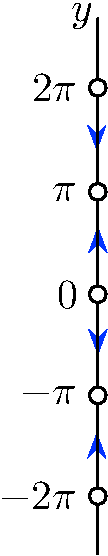
\includegraphics[height=150pt]{images/module14-equil1.pdf}
	\quad 
	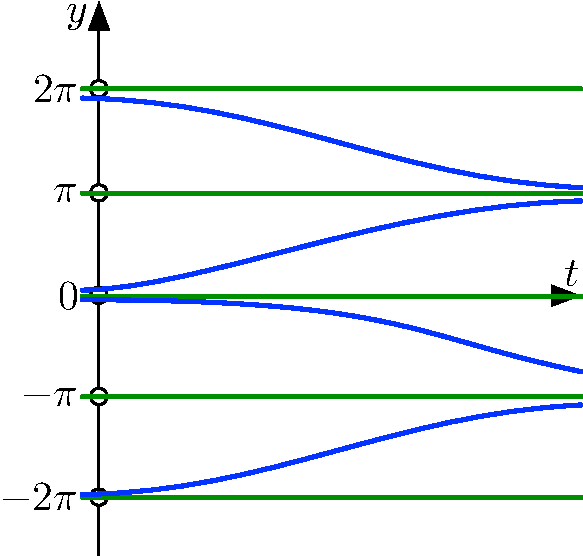
\includegraphics[height=150pt]{images/module14-equil2.pdf}
\end{center}

We can infer that the graphs will approach the constant solutions without touching because the derivative $y'$ will become smaller and smaller the more they approach the equilibria. We also know that solutions cannot touch each other.
\end{example}

There is also a distinction that we make about equilibrium points that helps us understand the behaviour of solutions. We will study this distinction in the core exercises.







\paragraph{\color{cyan}Population Models.} The fact that these differential equations keep the same rate of change independently of time, makes them an ideal candidate when studying populations.

%
%
%
%
%
%
%
%\paragraph{Exponential Growth. } 
%
%
%$P(t) = $ size of a certain population at time $t$
%
%\paragraph{Malthusian Population Model:}
%The population increases/decreases proportionally to its size, i.e.,
%$$
%\frac{dP}{dt} = rP,
%$$
%for some growth rate $r$.
%
%The solution of this DE is
%%    
%%    This is a separable $DE$, so we can solve it:
%%    \begin{align*}
%%    \frac{1}{P} \frac{dP}{dt} & = k \\
%%    \int \frac{1}{P} dP & = \int k dt \\
%%    \ln|P| &= kt + C \\
%%    |P| & = e^{kT+C} = e^C e^{kt} = A e^{kt}
%%    \end{align*}
%%    for $A = e^C >0$.
%%    
%%    So
%\[\tag{Review Exercise}
%P = P(0) e^{rt}.
%\]
%
%\begin{itemize}
%\item Population grows exponentially if $r>0$;
%\item Population decays exponentially if $r<0$.
%\end{itemize}
%
%This method is good while the environment can provide for all the population. Since there are no infinite environments, this method will ultimately fail! 
%
%
%\paragraph{Logistic Model:} Modification of the Malthusian model, to model an environment with limited resources. The individuals in the population are competing for resources among themselves:
%$$
%\frac{dP}{dt} = rP - \alpha P^2,
%$$
%where $P^2$ gives the number of possible encounters between individuals, and $\alpha$ gives a constant on how competition decreases the growth. 
%
%Another way to obtain this model is by observing that the rate of growth decreases as the population increases, so the simplest way to substitute $r$ with $r-\alpha P$ not the Malthusian Model. We obtain
%$$
%\frac{dP}{dt} = (r-\alpha P) P.
%$$
%
%Usually we write $\alpha = \frac rK$, so the model is
%\[\tag{Logistic Growth}
%\frac{dP}{dt} = r P \left(1 - \frac{P}{K}\right),
%\]
%for some intrinsic growth rate $r>0$ (the growth rate without limiting factors).
%
%This equation has two equilibrium solutions:
%$$
%P(t) = 0 \qquad \text{ and } \qquad P(t) = K.
%$$
%
%
%From the equation we observe the following: \\
%
%\begin{minipage}{10cm}
%\begin{itemize}
%\item The solutions cannot cross the line $y=K$: if they did, at $y=K$ they would have $y'=0$ and would remain at $y=K$
%
%\item Look the function $f(P) = \frac rK y(K-y)$ and analyze its sign:
%
%\item if $0<y(0)<K$, then $y' = f(y) > 0$, so the solution will keep increasing
%\item if $y(0)>K$, then $y' = f(y) < 0$, so the solution will keep decreasing
%
%\end{itemize}
%\end{minipage}
%\hfill
%\begin{minipage}{175pt}
%\includegraphics*[width=175pt]{figures/0205_auton.pdf}
%\end{minipage}
%
%\hfill\\
%
%We can now classify the equilibrium solutions:
%\begin{itemize}
%\item $P=0$ is unstable
%\item $P=K$ is stable
%\end{itemize}
%
%
%We can then conclude that the solutions will look like:
%\begin{center}
%\includegraphics*[width=150pt]{figures/0205_logpop.pdf}
%\end{center}
%
%\begin{rem}
%And the constant $K$ is the maximum number of individuals that the environment can sustain.
%\end{rem}
%
%
%We can solve this separable equation to obtain
%%
%%
%%\begin{gather*}
%%\frac{dP}{dt} = \frac rK P \left(K-P\right) \\
%%\frac{1}{P(K-P)} \frac{dP}{dt} = \frac rK \\
%%\\
%%\frac{1}{P(K-P)} = \frac AP + \frac{B}{K-P} \\
%%1 = A(K-P) + BP\\
%%AK=1\\
%%BK=1\\
%%\\
%%\left( \frac{1}{P} + \frac{1}{K-P}\right) \frac{dP}{dt} = r \\
%%\\
%%\ln|P| - \ln|K-P| = r t +C\\
%%\frac{P}{K-P} = c e^{rt} \\
%$$
%P(t) = \frac{K}{1+ce^{-rt}} 
%$$
%%\end{gather*}
%
%
%%
%%
%%To simplify the notation, we relabel the equation to
%%$$
%%\frac{dP}{dt} = P \left(a-bP\right),
%%$$
%%for $a,b>0$.
%%
%%
%%
%%This DE is separable, so we can solve it:
%%\begin{align*}
%%\frac{1}{P(a-bP)} \frac{dP}{dt} & = 1 \\
%%\int \frac{1}{P(a-bP)} dP & = \int 1 dt = t+C.
%%\end{align*}
%%
%%Using partial fractions, we write
%%\begin{align*}
%%\frac{1}{P(a-bP)}
%%	& = \frac{A}{P} + \frac{B}{a-bP} \\
%%	& = \frac{ A(a-bP) + BP}{P (a-bP)} \\
%%	& = \frac{ Aa + (B-Ab)P}{P (a-bP)}.
%%\end{align*}
%%
%%So $Aa = 1$ and $B-Ab = 0$. We have
%%$$
%%A = \frac{1}{a} \qquad \text{ and } \qquad B = \frac{b}{a}.
%%$$
%%
%%We now have
%%$$
%%\int \frac{1}{P(a-bP)} dP
%%	 = \int \frac{1}{a} \left(\frac{1}{P} + \frac{b}{a-bP}\right) dP
%%	 = \frac{1}{a} \left( \ln |P| - \ln |a-bP| \right)
%%	 = \frac{1}{a} \ln \left| \frac{P}{a-bP}\right|
%%$$
%%
%%The solution of the DE is given by
%%\begin{align*}
%%\frac{1}{a} \ln \left| \frac{P}{a-bP}\right| & = t+C \\
%%\ln \left| \frac{P}{a-bP}\right| & = at+aC \\
%%\left| \frac{P}{a-bP}\right| & = e^{aC}e^{at} = C_1 e^{at}
%%\end{align*}
%%for $C_1=e^{aC}>0$.
%%
%%We have
%%$$
%%\frac{P}{a-bP} =  \pm C_1 e^{at} = C_2 e^{at}.
%%$$
%%
%%Now we solve for $P$:
%%\begin{align*} 
%%P & = C_2 e^{at} (a-bP) \\
%%\left( 1 +C_2 b e^{at} \right) P & = C_2 a e^{at} \\
%%P & = \frac{C_2 a e^{at}}{1 +C_2 b e^{at}} \\
%%P & = \frac{a}{b + \frac{1}{C_2} e^{-at}}
%%\end{align*}
%%
%%We know that $\ds C_2 = \frac{P(0)}{a-bP(0)}$, so
%%$$
%%P(t) = \frac{a}{b + \left(\frac{a}{P(0)}-b\right) e^{-at}} 
%%= \frac{K}{1 + \left(\frac{K}{P(0)}-1\right) e^{-rt}}.
%%$$
%%
%%We can verify that $P(t) \to K$ as $t \to \infty$.
%\begin{note}
%We can improve on these models. For example, we can include a threshold of survivability, where if a population goes below that level, it will eventually become extinct.
%
%\subparagraph{Exercise. } Study the model
%$$
%\frac{dP}{dt} = -r\left(1-\frac PT\right) \left(1-\frac PK\right) P,
%$$
%where $r>0$ and $0<T<K$.
%\end{note}
%
%
%
%\paragraph{``Jelly Fish'' from MAT187. } 
%
%
%On a question of a midterm on MAT187, we studied another DE for a ``jelly fish'' population:
%$$
%\frac{dP}{dt} = r(P-T)(P-K)^2,
%$$
%for $0<T<K$.
%
%We can quickly study this problem qualitatively by studying the function: $f(y) =  r(y-T)(y-K)^2$.
%
%The equilibrium points are:
%$$
%T \quad , \quad K\quad .
%$$
%We study the sign of $f(y)$:
%
%\begin{center}
%\includegraphics*[width=200pt]{figures/0202_jellyfish.pdf}
%\hfil
%\includegraphics*[width=150pt]{figures/0202_jellyfish_sols.pdf}
%\end{center}
%
%We can also classify the equilibrium solutions:
%\begin{itemize}
%\item $P=T$ is unstable
%\item $P=K$ is semi-stable (stable from below and unstable from above)
%\end{itemize}
%
%
%And we can analyze the solutions:
%\begin{itemize}
%\item If $0< P_0 < T$, then the population will go extinct (in finite time). It doesn't just approach extinction asymptotically, it really does go extinct, as the slope keeps increasing (with negative sign)
%
%\item If $T<P<K$, then the population thrives and increases its number approaching $P=K$.
%
%\item If $T>K$, then the population increases at an accelerating pace. It goes ``viral''!
%\end{itemize}
%
%
%
%\subparagraph{Exercise. } Read Pages 81--83: Critical points and stable/unstable equilibrium solutions.



\begin{video}
\begin{itemize}
	\item \qrvideo{https://youtu.be/swt-let4pCI} %\href{https://youtu.be/swt-let4pCI}{https://youtu.be/swt-let4pCI} \hfill \qrcode{https://youtu.be/swt-let4pCI}
\end{itemize}	
\end{video}




	\begin{exercises}

	\begin{problist}
	\prob Show that all autonomous differential equations are separable.
	
	\prob Consider the ODE $y'=\displaystyle \frac1y$.
	Then which of the statements below are true or false and justify your choice.
	\begin{enumerate}
		\item The solutions always stay positive.
		\item The solutions always stay negative.
		\item The solutions never change sign.
		\item The solutions always change sign.
		\item Some solutions change sign, and some don't.
	\end{enumerate}
	
	\prob Sketch a slope field for the autonomous ODE $$y'=\cos(y).$$
	\prob Sketch a slope field for the autonomous ODE $$y'=\tan(y).$$
	\prob What is a common property of all slope fields of autonomous ODEs?
	
	
	\prob Consider the ODE
	$$ 
	y' = {\rm sign}(y) = 
		\begin{cases}
			1 & \text{ if } y > 0 \\	
			0 & \text{ if } y = 0 \\	
			-1 & \text{ if } y < 0
		\end{cases}. 
	$$

	\begin{enumerate}
		\item What are the equilibrium solutions?
		\item Find two solutions that satisfy $y(0)=0$.
		\item Are there solutions that satisfy $\displaystyle \lim_{t \to \infty} y(t) = \pi$?
		\item What are the possible limits of solutions as $t\to \infty$?
	\end{enumerate}
	
%		y=0 sol
%		y=max(0,t+c) sol
%		y=min(0,-t+c) sol




	\prob \label{mod14-q-stable}Consider a function $f(y)$ such that
	\begin{itemize}
		\item $f(1)=0$;
		\item $f'$ is continuous for all $y$;
		\item $f'(1)<0$.
	\end{itemize}
	\begin{enumerate}
		\item Show that there is an open interval $(a,b)$ satisfying $1 \in (a,b)$ and $f'(y)<0$ for all $y \in (a,b)$.
		\item Show that %there is an interval $(c,d) \subseteq (a,b)$ such that
		\begin{itemize}
%			\item $1 \in (c,d)$, 
			\item $f(y)>0$ if $y \in (a,1)$, %(c,1)$,
			\item $f(y)<0$ if $y \in (1,b)$. %(1,d)$.
		\end{itemize}
		\item Consider the initial-value problem $y'=f(y)$ with $y(0)=y_0$. Show that this problem has a unique solution.
		\item Show that if $y_0 \in (a,b)$, then $\displaystyle \lim_{t \to \infty} y(t) = 1$.
		\item Write a Theorem about equilibrium points based on the results of this question.
	\end{enumerate}


	\prob Consider a function $f(y)$ such that
	\begin{itemize}
		\item $f(2)=0$;
		\item $f'$ is continuous for all $y$;
		\item $f'(2)>0$.
	\end{itemize}
	
	Complete a study similar to question \ref{mod14-q-stable} for this function $f$.
	
	
	
	\prob Consider an autonomous ODE $y'=f(y)$ with two stable equilibrium solutions $y=1$ and $y=2$ and where $f$ is continuous.
	\begin{enumerate}
		\item Show that there must exist another equilibrium point $c \in (1,2)$.
		\item Show that if $f(y)\not\equiv 0$ in $(1,2)$, then there must exist an equilibrium point $c \in (1,2)$ that is either semi-stable or unstable.
	\end{enumerate}

	\end{problist}
\end{exercises}



%	\Heading{Motivation} 



\end{module}



\begin{lesson}
	\Title{Autonomous Differential Equations}

%	\Heading{Objectives}
%	\begin{itemize}
%		\item The second step in Mathematical modelling is to construct a representation of how the team will be attempting to solve the problem.
%		\item Create a mind map of the problem. This is a structured way to brainstorm possible solutions and their requirements.
%	\end{itemize}
%	
%	\Heading{Motivation} 
%
%\begin{annotation}
%	\begin{goals}
%	\Goal{Extra Reading}
%	Math Modelling: Getting started and getting solutions, Bliss-Fowler-Galluzzo
%	
%	\hfill \qrcode{https://m3challenge.siam.org/resources/modeling-handbook}	
%	\end{goals}
%\end{annotation}
%	\Heading{Extra Reading} \href{https://m3challenge.siam.org/resources/modeling-handbook}{Math Modelling: Getting started and getting solutions, Bliss-Fowler-Galluzzo}

\end{lesson}




\newpage

\question Consider the differential equation \quad $y'=f(y)$ \quad where $f(y)$ is given by the following graph:
\begin{center}
	\includegraphics*[width=350pt]{images/module14-graphf.pdf}
\end{center}

\begin{parts}
	\item What are the equilibrium points?
	\item Which equilibrium solutions are stable, unstable, or semi-stable?
	\item Write a definition for a \textbf{stable}, \textbf{unstable}, and \textbf{semi-stable} equilibrium point.
	\item Roughly, sketch a solution satisfying:
	\begin{enumerate}
		\item $y(0)=2.5$.
		\item $y(0)=-\frac14$.
		\item $y(1)=\frac14$.
	\end{enumerate}
	\item If $y(0) = 2$, then $y(t) = $
	\item If $y(0) = \frac12$, then $\displaystyle \lim_{t\to \infty} y(t) = $
	\item If $y(0) = -2$, then $\displaystyle \max_{t \in [0,\infty)} y(t) = $
\end{parts}


\bookonlynewpage


\hfill


\bookonlynewpage








